\section{Censoring-Aware Penetration Surrogate Modelling and Probabilistic Screening}

This chapter starts from the plume-resolved observables produced by the image-processing workflow and turns those discrete, partially censored measurements into trainable targets, an uncertainty-aware surrogate, and a simplified geometric screening proxy. The split between ``video to observables'' and ``observables to predictor'' is intentional, so that the assumptions and limits of each layer can be inspected separately.

Short pilot injections sharpen the tension between measured traces and trainable targets.
Classical empirical penetration laws remain physically valuable, but their applicability narrows when the observable window is dominated by start-of-injection and end-of-injection transients.
The right-censoring issue established in Chapter~2 is treated here as a target-construction constraint that propagates into the fitting, uncertainty, and distillation stages.

\subsection{Problem reframing and observable contract}
\label{sec:surrogate-problem-framing-en}

The modelling task in this chapter is deliberately framed as a low-dimensional probabilistic regression problem rather than as a raw-image prediction problem. Chapter~3 has already converted the top-view Mie recordings into plume-resolved temporal observables. The surrogate therefore receives operating-condition and geometry descriptors, together with time, and predicts a conditional penetration distribution,
\[
x=\{t,\theta_{\mathrm{tilt}},N_{\mathrm{plume}},t_{\mathrm{inj}},P_{\mathrm{cb}},P_{\mathrm{inj}},P_{\mathrm{ch}},d_n,\rho_a\}
\;\longmapsto\;
\{\mu_S(t),\sigma_S(t)\}.
\]
The scalar target \(S(t)\) is measured in millimetres, while \(\sigma_S(t)\) is interpreted as a heteroscedastic conditional spread rather than as a single global residual band.

Among the penetration descriptors exported by the image-processing workflow, CDF penetration is used as the primary training and evaluation observable. The binary axial penetration \(S_{\mathrm{BW,x}}\) and polar/boundary penetration proxy \(R_{\mathrm{BW}}\) remain important consistency checks and geometry diagnostics, but they inherit thresholding, morphology, and boundary-interpretation choices from the binary support image. The CDF front instead follows the axial cumulative support of the cleaned plume strip, making it less sensitive to isolated leading pixels and more directly aligned with the time-series target needed by the surrogate. Consequently, all training and evaluation protocols below are stated in the CDF penetration convention unless explicitly marked otherwise.

This reframing also fixes the role of uncertainty. The goal is not merely to fit a smooth mean curve through every measured point; the downstream screening task needs a distribution over plausible penetration at each time. The chapter therefore treats the archive in three complementary ways: as a collection of raw time-indexed measurements, as a statistically truncated point-level evaluation set, and as a fitted trajectory archive that can serve as a smooth teacher. The rest of the chapter defines those populations, constructs the fitted target, and then compares neural and kernel-based backbones for the same scaled regression problem.

\subsection{CDF censoring and three derived data populations}
\label{sec:cdf-populations-en}

\subsubsection{Spatial right-censoring audit of the CDF penetration traces}
\label{sec:cdf-spatial-censoring-audit}
\newcommand{\scrNTotal}{24316}%
\newcommand{\scrNCensored}{9630}%
\newcommand{\scrRatePct}{39.6}%
\newcommand{\scrNaiveHoldGapMedianMm}{46}%

Before constructing fitted targets, the severity of the CDF penetration right-censoring problem is quantified directly from the image-processing outputs. This audit defines censoring spatially rather than from the later \(\SI{5}{ms}\) surrogate horizon. For each nozzle family \(n\), all positive raw CDF penetration values exported by the multi-hole Mie workflow are pooled and a field-of-view cap \(C_n\) is estimated as the \(q=0.999\) quantile. A plume trajectory is then marked as spatially right-censored if its raw or cleaned CDF trace reaches \(C_n-\epsilon_n\), with \(\epsilon_n=\max(\SI{1}{mm},0.01C_n)\). The audit is implemented in the spatial right-censoring audit script, comparing the raw Mie outputs in the Mie image-processing output directory with the fitted targets in the synthetic data export directory (codebase identifiers are tabulated in Appendix~\ref{app:implementation_mapping}).

The resulting scalar diagnostic is the spatial censoring rate,
\[
\mathrm{SCR}
=
\frac{1}{N}\sum_{i=1}^{N}
\mathbf{1}\!\left[
\max_t S_i^{\mathrm{raw/clean}}(t)
\ge C_{n(i)}-\epsilon_{n(i)}
\right],
\]
where \(n(i)\) is the nozzle family of trajectory \(i\).

The clean split contains \(\num{\scrNTotal}\) CDF penetration trajectories, of which \(\num{\scrNCensored}\) meet this spatial right-censoring criterion, giving a spatial censoring rate of \(\scrRatePct\%\). The median nozzle-specific cap is \(\SI{92.52}{mm}\). Among censored clean trajectories, the median first cap hit occurs at \(\SI{1.76}{ms}\), corresponding to \(44.4\%\) of the raw positive observation span. If a naive target construction simply held the final cleaned CDF penetration value forward, its median gap relative to the accepted q1 continuation at \(\SI{5}{ms}\) would be approximately \(\SI{\scrNaiveHoldGapMedianMm}{mm}\); if the cap itself were treated as the terminal saturation value, the corresponding median gap would still be \(\SI{43.96}{mm}\). These continuation gaps are not treated as wide-field ground-truth errors. They quantify the size of the target bias that would be introduced by reading cap-hit traces as physically saturated observations.

\begin{figure}[t]
\centering
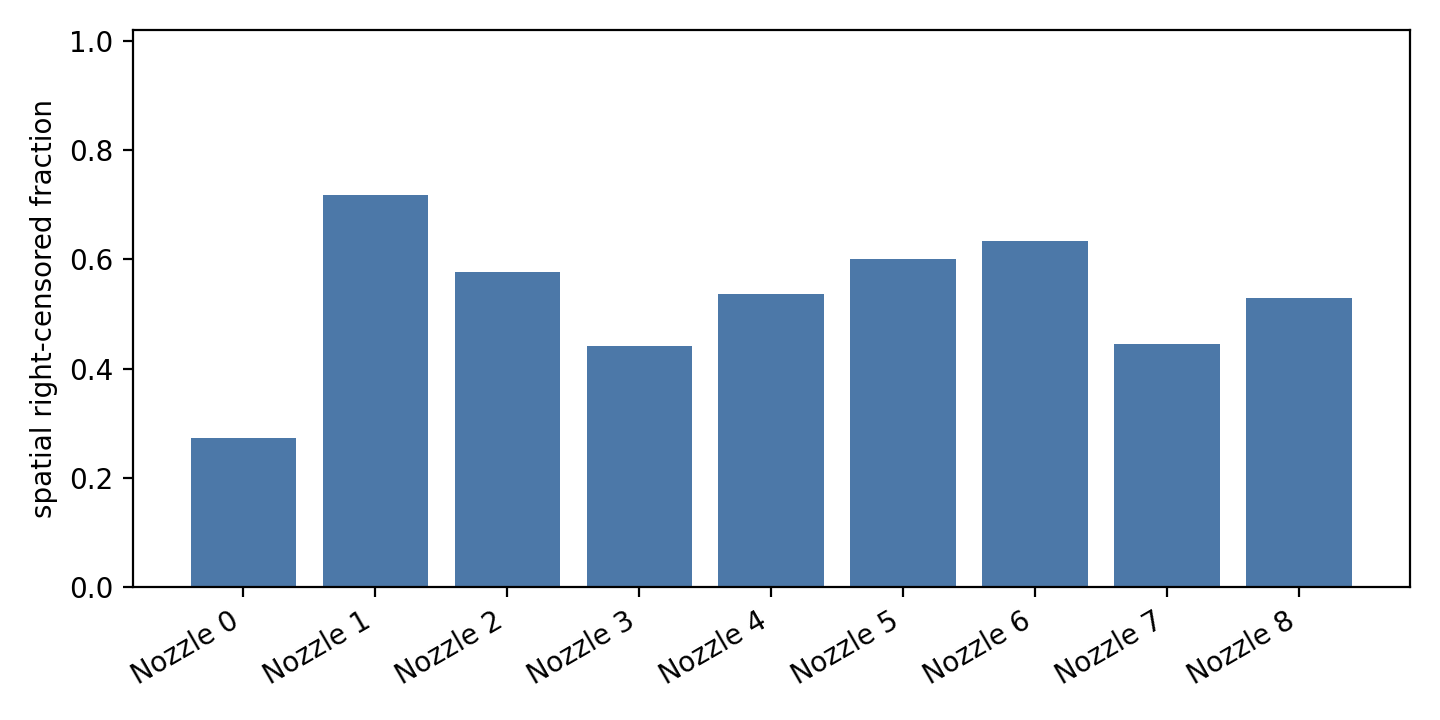
\includegraphics[width=0.88\linewidth]{images/fig_spatial_censoring_fraction_by_nozzle_clean.png}
\caption{Nozzle-wise spatial right-censoring fraction for the clean CDF penetration trajectories. The nozzle-specific cap varies across families because each nozzle campaign was conducted under a distinct optical configuration — camera standoff and lateral positioning were not held constant between nozzle groups, though they were consistent within each family. Nozzle family therefore acts as an indirect proxy for the field-of-view limit. A trajectory is counted as censored when its raw or cleaned CDF penetration reaches the nozzle-specific field-of-view cap estimated from raw Mie outputs. The audit shows that the cap-hit problem is not restricted to a small tail of the archive: approximately \(\scrRatePct\%\) of clean CDF penetration trajectories are spatially censored overall.}
\label{fig:spatial-censoring-by-nozzle-clean}
\end{figure}

\begin{table}[t]
\centering
\footnotesize
\begin{tabular}{@{}L{0.58\linewidth}L{0.34\linewidth}@{}}
\toprule
Audit quantity & Clean CDF penetration split \\
\midrule
Total trajectories & \(\num{\scrNTotal}\) \\
Spatially right-censored trajectories & \(\num{\scrNCensored}\) (\(\scrRatePct\%\)) \\
Median nozzle-specific cap & \(\SI{92.52}{mm}\) \\
Median first cap-hit time among censored traces & \(\SI{1.76}{ms}\) \\
Median cap-hit position within raw positive span & \(44.4\%\) \\
Median naive-hold gap relative to q1 continuation & \(\SI{\scrNaiveHoldGapMedianMm}{mm}\) \\
Median cap-saturation gap relative to q1 continuation & \(\SI{43.96}{mm}\) \\
\bottomrule
\end{tabular}
\caption{Spatial censoring audit summary for clean CDF penetration trajectories. The two continuation-gap rows compare naive censored-target constructions with the accepted q1 continuation at \(\SI{5}{ms}\); they are used as target-bias diagnostics rather than as direct measurement error against unavailable wide-field truth.}
\label{tab:spatial-censoring-audit-clean}
\end{table}

This audit makes the modelling consequence explicit. The raw CDF penetration traces handed over by Chapter~3 are not merely short or noisy; a large fraction reach a nozzle-specific spatial limit well before the time horizon used by the surrogate targets. The reduced-order continuation, the heteroscedastic teacher, and the later raw/KD regime split are therefore responses to a quantified observation problem rather than optional modelling embellishments.

\subsubsection{Three derived populations from the cleaned CDF archive}
\label{sec:three-derived-populations-en}

The cleaned CDF archive is not consumed as a single homogeneous dataset. Downstream code reads it through three structurally distinct populations, each with its own selection bias and role in the surrogate protocol.

\textbf{Dataset \#1: raw cleaned CDF observations.}
This population consists of the per-frame \((t,S)\) observations that survive the Chapter~3 CDF extraction, hydraulic-delay alignment, jump truncation, and short-segment filtering. It is stored in long and wide forms under the cleaned CDF series exports. The clean archive contains approximately \(24{,}316\) accepted trajectories and \(703{,}592\) individual frame observations. Its strength is pointwise fidelity: these rows are the closest object in the pipeline to the measured penetration record, and they preserve the time-dependent noise and plume-to-plume scatter. Its limitation is the censoring quantified above: late bins are depleted by FOV hits and signal decay, so raw supervision is trustworthy only while coverage remains high. Stage~3 therefore uses this population directly only in the reliable raw-CDF regime.

\textbf{Dataset \#2: statistically truncated points and the P50/q1 oracle.}
This population is derived from Dataset~\#1 by aggregating observations within each operating condition. The point-level table bins time in \(\Delta t=\SI{0.1}{ms}\) intervals over \(0\)--\(\SI{5}{ms}\), then truncates each condition at the first bin satisfying either a density-drop criterion or an FOV-saturation criterion: the smoothed per-bin trajectory count falls below a fixed fraction of its within-condition peak, or the per-bin \(p_{95}\) penetration reaches \(95\%\) of the estimated FOV cap. The resulting uncensored point set contains approximately \(506{,}634\) points across \(592\) operating conditions. A companion P50/q1 oracle is built by taking the per-bin median penetration for each retained condition and fitting q1 to that median trace; it covers \(495\) conditions and provides a condition-level reference curve. This dataset is not used for training. It is a less-biased evaluation ruler for uncensored CDF accuracy, P50 observed behaviour, Q1 extrapolation diagnostics, LONO evaluation, and the MLP--SVGP comparison.

\textbf{Dataset \#3: per-trajectory q1 fitted archive.}
For each accepted plume trajectory, the reduced-order q1 model described in Section~\ref{sec:q1-target-construction-en} stores the fitted parameters and associated fit diagnostics. This population provides smooth, differentiable, extrapolable targets over the surrogate horizon. Stage~1 selects one representative fitted trajectory per operating-condition group from this population, and Stage~2 trains on all filtered fitted trajectories that pass the robust post-fit gates. The same filtering makes Dataset~\#3 useful as a clean teacher source but also gives it a clear selection bias: it favours optically clean, monotone, q1-representable trajectories.

\begin{table}[t]
\centering
\footnotesize
\setlength{\tabcolsep}{3pt}
\begin{tabular}{@{}L{0.25\linewidth}L{0.22\linewidth}L{0.22\linewidth}L{0.22\linewidth}@{}}
\toprule
Pipeline role & Dataset \#1: raw CDF points & Dataset \#2: uncensored / P50 reference & Dataset \#3: q1 fitted archive \\
\midrule
Primary artefact & \codepath{series\_clean} and \codepath{series\_wide\_clean} & \codepath{cdf\_points\_uncensored.csv} and P50/q1 oracle tables & \codepath{clean/*.csv} q1 fit tables \\
\midrule
Stage~1 training & --- & --- & representative q1 trajectories \\
Stage~2 training & --- & --- & filtered q1 trajectories \\
Stage~3 raw supervision & reliable-coverage bins & --- & indirect, through the Stage~2 teacher \\
\midrule
Main evaluation role & full-clean diagnostic & uncensored CDF, P50, Q1, LONO, MLP--SVGP comparison & in-domain fitted-target diagnostics \\
\bottomrule
\end{tabular}
\caption{Three derived populations read from the cleaned CDF penetration archive. Dataset~\#1 is the closest pointwise measurement record, Dataset~\#2 is the less-biased evaluation ruler, and Dataset~\#3 is the smooth fitted-target archive used by Stage~1 and Stage~2.}
\label{tab:three-derived-populations}
\end{table}

The distinction between the Stage~1 representative trajectory and the P50/q1 oracle is especially important. The Stage~1 row is one real q1-fitted trajectory drawn from Dataset~\#3: within each operating-condition group, the fitted curve is evaluated at \(\SI{5}{ms}\), the group median is computed, and the nearest real trajectory is kept. The P50/q1 oracle is a virtual trajectory built from Dataset~\#2 by taking the per-time-bin median and then fitting q1 to that median trace. The former is a training target and inherits Dataset~\#3's robust-z filtering; the latter is an evaluation reference and never enters training.

\subsection{Censoring-aware q1 target construction}
\label{sec:q1-target-construction-en}

\subsubsection{Trajectory cleaning and time alignment}

The learned models do not train directly on the raw exported traces. Instead, the cleaning and fitting routine first cleans and time-aligns them. For each plume, the routine finds the earliest valid penetration segment, takes the first two positive samples after onset, fits a straight line to those early nonzero points, and uses the \(x\)-axis intercept of that line as a subframe opening-delay estimate whenever the fitted slope is positive. If an area-based onset marker is available, that frame anchors the delay scan; otherwise it falls back to the first positive penetration frame. The resulting raw delay is then clipped to a small median-centred window across plumes so that one anomalous plume does not over-shift the whole group.

That delay estimate is used in two coupled ways. The penetration array itself is shifted left by the nearest integer number of frames, while the aligned time vector retains the fractional residual through the exact offset subtraction. The pipeline performs a plume-onset registration that preserves subframe timing information before the later reduced-order fit. After alignment, sudden unrealistic jumps are removed, and low-quality fits are flagged through a set of rule-based masks.

\subsubsection{Two-regime candidate model}

Hiroyasu and Arai divide diesel spray penetration into two stages---pre-breakup (\(\sqrt{t}\) dominant) and post-breakup (\(t^{1/4}\) dominant) \cite{HiroyasuArai1990}---and the two-branch candidate model in this section builds directly on that framework. Two adaptations are made: a differentiable sigmoid gate replaces the hard staged switch, giving a smooth differentiable fitted curve; and the fit is kept free of any external physical quantities beyond the penetration observations themselves, so that each trajectory can be fitted independently. Later work on start-of-injection transients further shows that short injections are difficult to cover with a single rigid empirical expression over the entire trace \cite{ZhouLiYi2021}, a consideration that is especially prominent here because the present experiments use pilot diesel injection, where the near-SOI segment is short, highly transient, and has a relatively low signal-to-noise ratio.

Each accepted trajectory is then fitted with a smooth two-regime model,
\[
S(t)=\left(1-w(t)\right)k_{\mathrm{sqrt}}\sqrt{t}
+w(t)k_{\mathrm{quarter}}t^{1/4},
\qquad
w(t)=\sigma\!\left(\frac{t-t_0}{s}\right),
\]
where \(k_{\mathrm{sqrt}}\), \(k_{\mathrm{quarter}}\), \(t_0\), and \(s\) are optimized in log space. Concretely, the fitting problem is posed as a robust nonlinear least-squares estimation,
\[
\min_{\theta}
\sum_i \rho_\delta\!\left(S(t_i;\theta)-y_i\right),
\qquad
\theta=
\left[\log k_{\mathrm{sqrt}},\log k_{\mathrm{quarter}},\log t_0,\log s\right],
\]
with the Huber penalty
\[
\rho_\delta(r)=
\begin{cases}
\tfrac{1}{2}r^2, & |r|\le \delta,\\
\delta\left(|r|-\tfrac{1}{2}\delta\right), & |r|>\delta.
\end{cases}
\]
where \(r = S(t_i;\theta)-y_i\) is the fitting residual and \(\delta\) is the threshold where the penalty transitions from squared-error to absolute-error. The objective is solved by trust-region nonlinear least squares with \(\delta=1\), while the log-parameterization keeps the fitted gains and transition scale positive \cite{Huber1964,NocedalWright2006}.
The model should therefore be read as a temporal parameterization rather than as an explicit physics law. Its purpose is twofold: to provide believable extrapolation farther from EOI, where the downstream surrogate needs stable targets, and to provide acceptable interpolation near SOI, where the relative error is larger and the apparent early-time physics are harder to constrain from the image trace alone. The sigmoid gate is important for that role. Instead of imposing a hard breakpoint between two empirical branches, it creates a differentiable transition, which keeps the fitted curve smooth and makes it more compatible with the later neural-network stage. In other words, the early transient physics are not forced into a rigid closed-form law here; they are only approximated well enough that the subsequent network can learn the remaining condition-dependent behaviour from the full operating-point inputs.

This interpretation becomes clearer when the fit is compared with the extended EOI expressions in the spray literature. The Zhou et al.\ post-EOI model distinguishes the global injection clock \(t\) from the delayed clock \((t-t_i)\), because the late penetration branch is activated only after the end-of-injection dynamics have propagated downstream \cite{ZhouLiLaiWei2019}. The present pipeline handles that delay in two layers. First, the preprocessing stage estimates a plume-wise onset delay from the early linear extrapolation described above and shifts the observed series toward a common \(t\approx 0\) reference. Second, the reduced-order fit itself still does not contain an explicit delayed clock inside the parametric branch. Instead, it uses
\[
w(t)=\sigma\!\left(\frac{t-t_0}{s}\right)
\]
to suppress the quarter-root branch before a learned transition time \(t_0\), and then allows the \(t^{1/4}\) term to dominate only after that transition. This is not algebraically identical to replacing \((t-t_i)^{1/4}\) with \(t^{1/4}\). Rather, it is an engineering reparameterization: on a finite observation window, a delayed fourth-root branch can often be represented adequately by a gated unshifted fourth-root branch with adjusted amplitude and transition location, especially when the early part of that branch is strongly attenuated by \(1-w(t)\) or \(w(t)\) near zero. In that sense, the delayed physical clock is absorbed into the learned switching parameters \((t_0,s)\) and into the branch amplitudes rather than being imposed as a fixed known constant.

The engineering approach is therefore considered reasonable for the stated objective of this thesis, with one explicit boundary. It is reasonable because the fit is used as a smooth compressor of noisy trajectories, not as a final mechanistic spray law; it keeps the curve differentiable for later learning; and it leaves the operating-condition dependence to the neural network instead of forcing every physical effect into the closed-form fit. The boundary is that this justification should be presented as a reduced-order surrogate motivated by empirical penetration theory, not as proof that the shifted-time physics have disappeared. The quarter-root-only ablation below makes the comparison explicit.

\subsubsection{Quarter-root dominance and selection of the q1 production model}

If \(k_{\mathrm{sqrt}}\) is nearly zero in practice, retaining that degree of freedom is not merely redundant --- it may actively harm performance on difficult trajectories. A quantitative check across all accepted fits directly confirms the former; the ablation below confirms the latter.

A direct quantitative check across the \(14{,}563\) accepted plume fits in the polar binary penetration archive confirms this conclusively. At the fitted transition time \(t_0\), the two branch amplitudes are \(k_{1/4}\cdot t_0^{1/4}\) (quarter-root) and \(k_{\mathrm{sqrt}}\cdot t_0^{1/2}\) (square-root); their ratio is
\[
r = \frac{k_{\mathrm{sqrt}}\cdot t_0^{1/4}}{k_{1/4}}.
\]
Across all accepted fits, the median ratio is \(r_{\mathrm{med}}=2.9\times10^{-9}\), with an interquartile range of \([9.0\times10^{-10},\;1.1\times10^{-8}]\). In \(99.8\%\) of accepted fits, \(r<0.5\); in \(100\%\), \(r<1\). Expressed as absolute amplitudes, the median quarter-root branch contributes \(\SI{69.2}{mm}\) at \(t_0\), while the median square-root branch contributes \(2.0\times10^{-7}\,\si{mm}\)---a difference of eight orders of magnitude. Figure~\ref{fig:ksqrt-ratio} shows the full distribution of \(\log_{10}(r)\) (panel~a) and the quarter-root amplitude distribution (panel~b). In practice, the square-root term is negligible at the transition time for every fit in this archive, so the successful fits degenerate entirely toward a quarter-root-dominated curve. This is acceptable for the intended use: the physical drivers are later given directly to the neural network, while the fit itself remains self-adaptive and physics-light.

\begin{figure}[t]
\centering
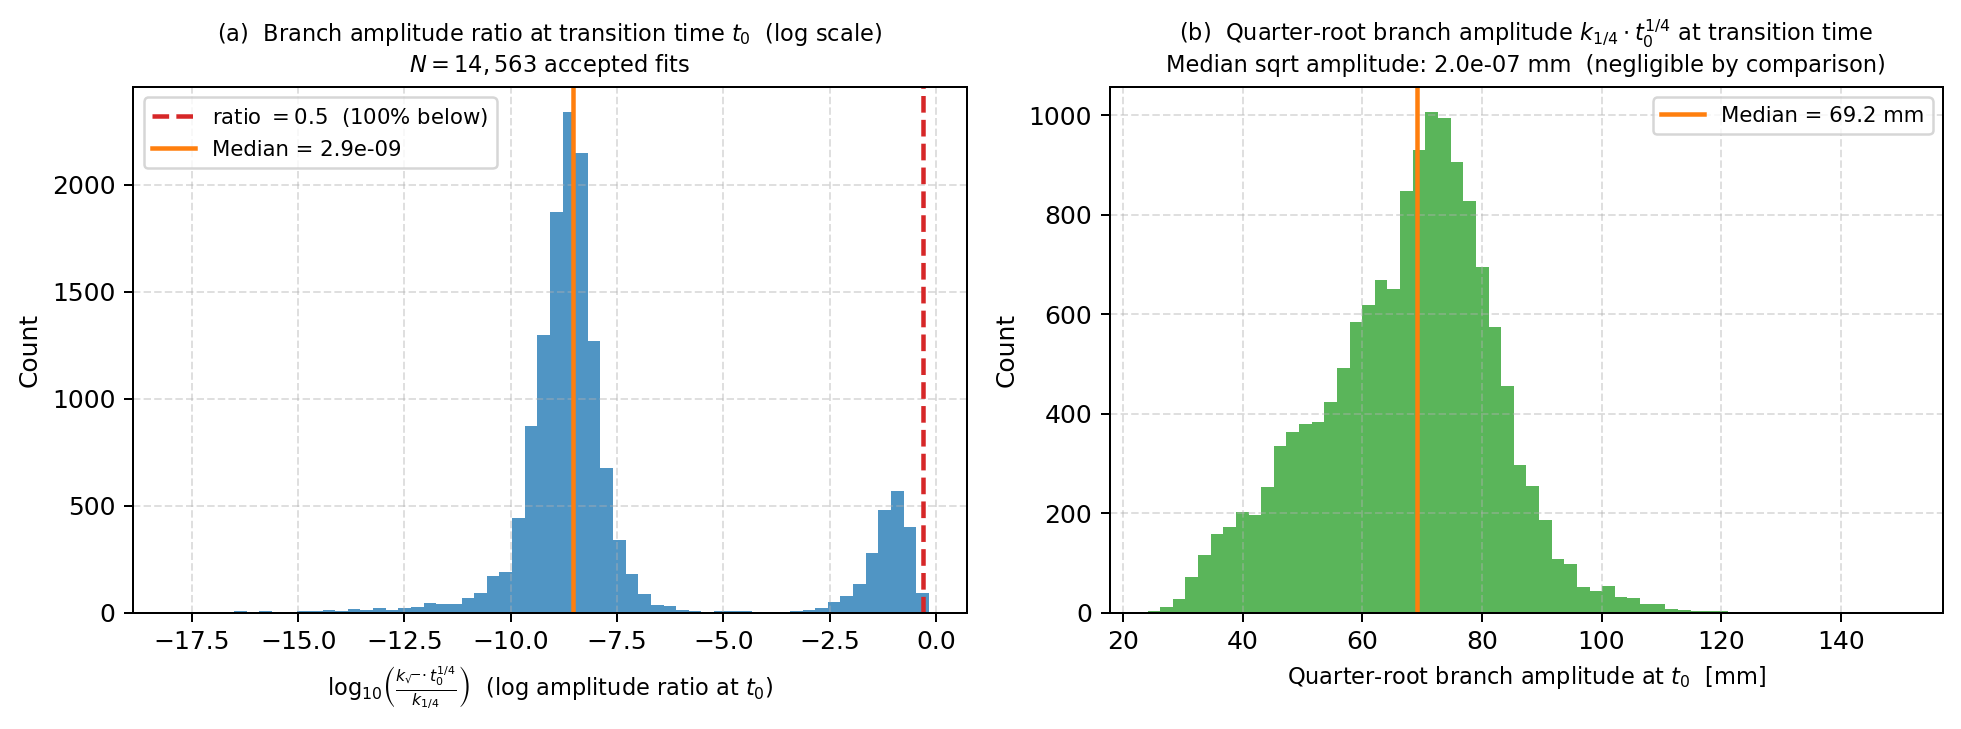
\includegraphics[width=0.96\linewidth]{images/ksqrt_ratio_distribution.png}
\caption{Quantitative assessment of the square-root branch weight across \(14{,}563\) accepted plume fits (clean-fit archive, the polar binary penetration metric source). (a)~Log-scale distribution of the branch amplitude ratio \(r=k_{\mathrm{sqrt}}\cdot t_0^{1/4}/k_{1/4}\) at the fitted transition time; the red dashed line marks \(r=0.5\) (99.8\% of fits fall below). (b)~Quarter-root branch amplitude distribution; its median of \SI{69.2}{mm} is eight orders of magnitude larger than the corresponding square-root branch, confirming that virtually all accepted fits are quarter-root dominated.}
\label{fig:ksqrt-ratio}
\end{figure}

This observation directly motivates a structural ablation: if successful fits already converge to a quarter-root-dominated curve, the residual \(k_{\mathrm{sqrt}}\) freedom may act as a destructive degree of freedom on harder traces. When the solver cannot find a well-constrained minimum on a short or noisy trajectory, the unchecked \(\sqrt{t}\) term can grow during optimisation and drive the far-time extrapolation to physically implausible values, so that the masking pipeline rejects the series even though the quarter-root component alone might have fitted it adequately.

The reduced single-branch model, referred to as q1 (for quarter-root, single branch), eliminates this risk by replacing the two-regime blend with a single sigmoid-gated quarter-root branch,
\[
S_{q1}(t) = \sigma\!\left(\frac{t-t_0}{s}\right)\,k_{1/4}\,t^{1/4},
\]
reducing the parameter count from four to three: \([\log k_{1/4},\,\log t_0,\,\log s]\). An equivalent masking pipeline is constructed for q1 in parallel: the fitted curve is evaluated at \(t_{\mathrm{far}}=\SI{5}{ms}\) and checked against the same physical plausibility window \([18,\,300]\,\si{mm}\); the same \(t_0 < \SI{0.8}{ms}\) and \(s < \SI{1}{ms}\) bounds are applied; and the same grouped robust-\(z\) outlier scores are computed on \(t_0\), RMSE, and cost-per-point. A series is counted as successfully fitted when it passes the complete masking pipeline and additionally satisfies \(\mathrm{RMSE} < \SI{3}{mm}\), making the two success criteria symmetric and directly comparable.

Across all \(23{,}495\) series in the nine-nozzle CDF penetration campaign (after discarding series shorter than ten valid frames), the four-parameter main model achieves a success rate of \(61.3\%\), while the q1 model achieves \(90.0\%\)---an absolute gain of 28.6~percentage points with no individual nozzle regressing. On the clean subset that passes both models, the median RMSE is \(\SI{1.23}{mm}\) for the main model and \(\SI{1.27}{mm}\) for q1, confirming that removing \(k_{\mathrm{sqrt}}\) costs nothing on well-behaved data. On the flagged subset the contrast is far more pronounced: the median RMSE drops from \(\SI{8.12}{mm}\) to \(\SI{1.08}{mm}\), a reduction of approximately \(7.5\times\). The gain is largest for the most heavily impinged datasets---Nozzle0 improves by 37.6 percentage points and Nozzle~7 by 28.7 percentage points---which are precisely the conditions where the post-impingement deceleration phase makes the \(t^{1/4}\) form the dominant descriptor and renders the \(\sqrt{t}\) branch physically uninformative.

Based on this ablation, q1 is promoted to the production fitting target, and the smooth targets consumed by Stage~1, Stage~2, and Stage~3 are all produced by q1 rather than by the four-parameter candidate model. The four-parameter results are retained only as a structural diagnostic and as a historical baseline that motivates the reduced-order step. The practical purpose of this fit is therefore not to claim a universal penetration law, but to compress noisy plume trajectories into smooth, differentiable, and trainable targets while preserving the dataset's heteroscedastic variation for the later learning stages.

\subsubsection{q1 diagnostics: scaling, residuals, and identifiability}

\textbf{Empirical scaling check.} A post-hoc scaling regression on the \(24{,}316\) accepted q1 fits provides a sanity check against classical penetration theory. Fitting \(\log k_{1/4} = a\,\log\Delta P + b\,\log\rho_a + c\,\log d_n + \text{const}\) by ordinary least squares yields exponents \(a\approx 0.52\), \(b\approx -0.23\), \(c\approx 0.26\) with \(R^2\approx 0.27\). The \(\rho_a\) exponent matches the Hiroyasu--Arai post-breakup form \(S\propto\Delta P^{1/4}\rho_a^{-1/4}(d_n t)^{1/2}\) almost exactly at \(-1/4\). The injection-pressure exponent (\(a\approx 0.52\)) is noticeably steeper than the Hiroyasu--Arai value of \(1/4\); the reason for this discrepancy is not certain, and several causes — including the dataset's condition coverage, the functional form of the q1 fit, and the fact that the \(t^{1/4}\) branch may absorb more than the free-jet stage — would each be consistent with the observation. The diameter exponent (\(c\approx 0.26\)) sits well below the classical \(1/2\), most likely reflecting collinearity between nozzle diameter and other operating conditions in the experimental matrix (Section~\ref{sec:pointlevel-scaling-verification} confirms this independently). Regressions on the gating parameters \(t_0\) and \(s\) yield much lower \(R^2\) (\(0.17\) and \(0.14\)), which is expected: a sigmoid switching time is not directly predicted by Hiroyasu--Arai theory and absorbs the residual onset-delay variability left after preprocessing alignment.
As a cross-check, regressing \(\log S\) directly on the raw discrete observations at fixed \SI{0.1}{ms} time bins yields a log-log \(R^2\) of approximately \(0.47\)--\(0.51\) in the mid-trajectory window (\(0.35\)--\(0.75\)~ms), confirming that the three physical variables explain a meaningful fraction of raw penetration variance in the well-sampled regime. The lower \(R^2\approx 0.27\) obtained from the compressed \(k_{1/4}\) parameter reflects integration across the noisy onset and post-injection regimes rather than model failure; the chamber-pressure exponent (\(\approx-0.25\)) and the qualitative trend of the \(\Delta P\) exponent (\(0.44\)--\(0.65\), intermediate between the Bernoulli value of \(0.5\) and the H--A value of \(0.25\)) are consistent across both analyses.

\begin{figure}[t]
\centering
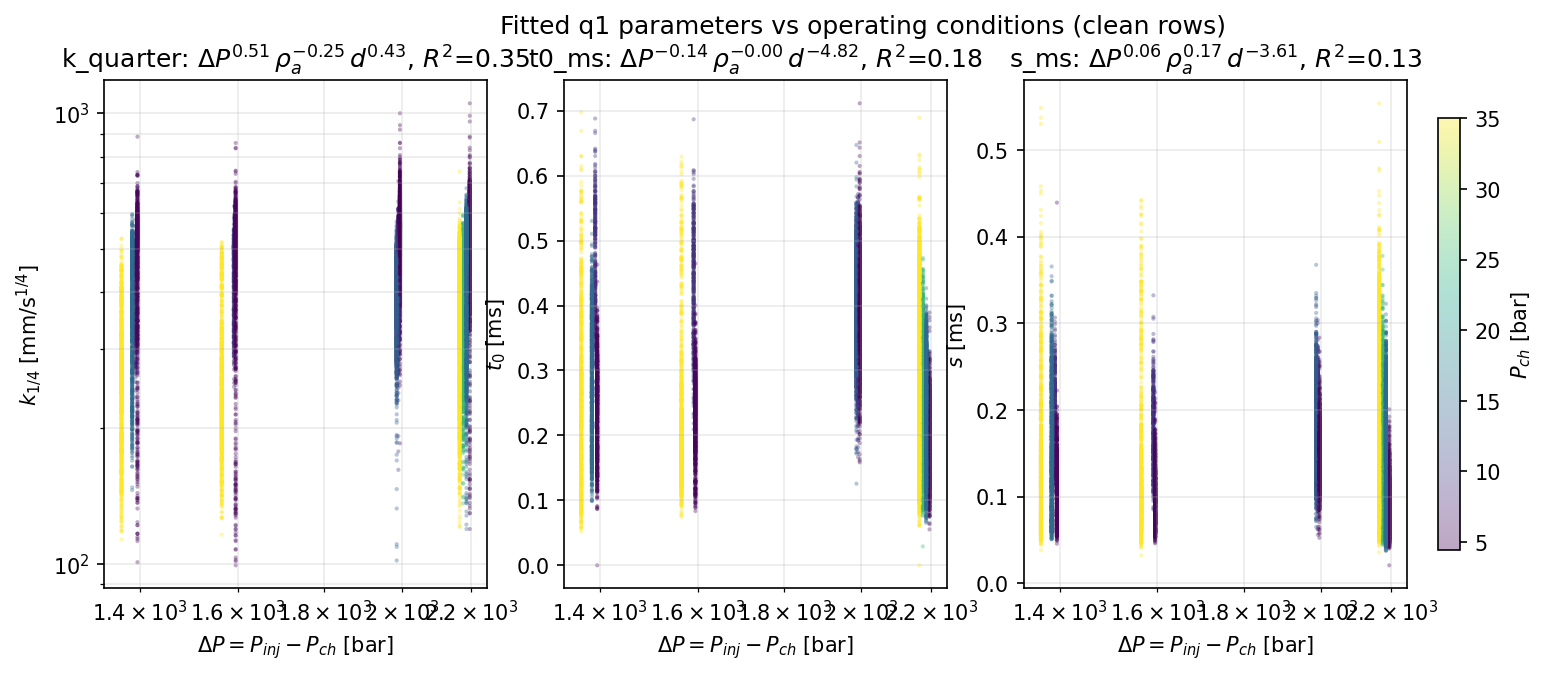
\includegraphics[width=0.96\linewidth]{images/fig_q1_param_scaling.png}
\caption{Empirical scaling of the q1 production parameters \((k_{1/4},t_0,s)\) against \(\Delta P=P_{\mathrm{inj}}-P_{\mathrm{ch}}\), colour-coded by chamber pressure \(P_{\mathrm{ch}}\). Each panel title reports the fitted log-log exponents and \(R^2\) of the regression \(\log y = a\log\Delta P + b\log\rho_a + c\log d_n + \text{const}\). The \(k_{1/4}\) panel shows that \(\rho_a^{-0.23}\) closely matches the Hiroyasu--Arai expectation of \(-1/4\), while the diameter exponent (\(d_n^{0.26}\)) falls noticeably below the classical \(1/2\); the gating parameters are weakly explained by the same dimensional group.}
\label{fig:q1-param-scaling}
\end{figure}

\textbf{Residual structure and heteroscedasticity.} Reconstructing the residual \(\hat S(t)-y(t)\) for every clean fit at every observed frame, then binning by \(\Delta t=\SI{0.1}{ms}\), produces the empirical envelope in Figure~\ref{fig:q1-residual-structure}. The diagnostic reveals two distinct regimes. In the central window \(t\in[0.3, 1.0]\,\si{ms}\) the median residual stays below \(\SI{0.4}{mm}\) and the robust spread \(\sigma_{\mathrm{robust}}(t)=1.4826\,\mathrm{MAD}(t)\) reaches a minimum of \(\sim\SI{0.60}{mm}\) near \(t=\SI{1.0}{ms}\), so q1 is essentially unbiased and tight in the well-sampled mid-trajectory. Both boundaries inflate the residuals: the very first bin at \(t=\SI{0.05}{ms}\) carries a positive bias of \(\sim\SI{+1.7}{mm}\) with \(\sigma_{\mathrm{robust}}\approx\SI{1.8}{mm}\), reflecting onset-alignment imprecision and the steep sigmoid gate transition near \(t_0\); the late tail at \(t=\SI{1.55}{ms}\) carries a negative bias of \(\sim\SI{-1.6}{mm}\) with \(\sigma_{\mathrm{robust}}\approx\SI{0.7}{mm}\), reflecting right-censoring of the surviving population (per-bin counts collapse from \(\sim 65{,}000\) frames at \(t=\SI{0.15}{ms}\) to fewer than \(200\) at \(t=\SI{1.55}{ms}\)). The envelope is therefore U-shaped rather than monotonically growing, but the implication for the surrogate stack is the same either way: the residual scale is strongly time-dependent, so a fixed-variance loss is inappropriate and Stage~2 must learn an input-dependent \(\sigma\) rather than a single scalar. The Stage-1 deterministic baseline captures the \emph{conditional mean} this diagnostic exposes, while Stage~2 is responsible for the \emph{conditional spread}, including its boundary inflation.

\begin{figure}[t]
\centering
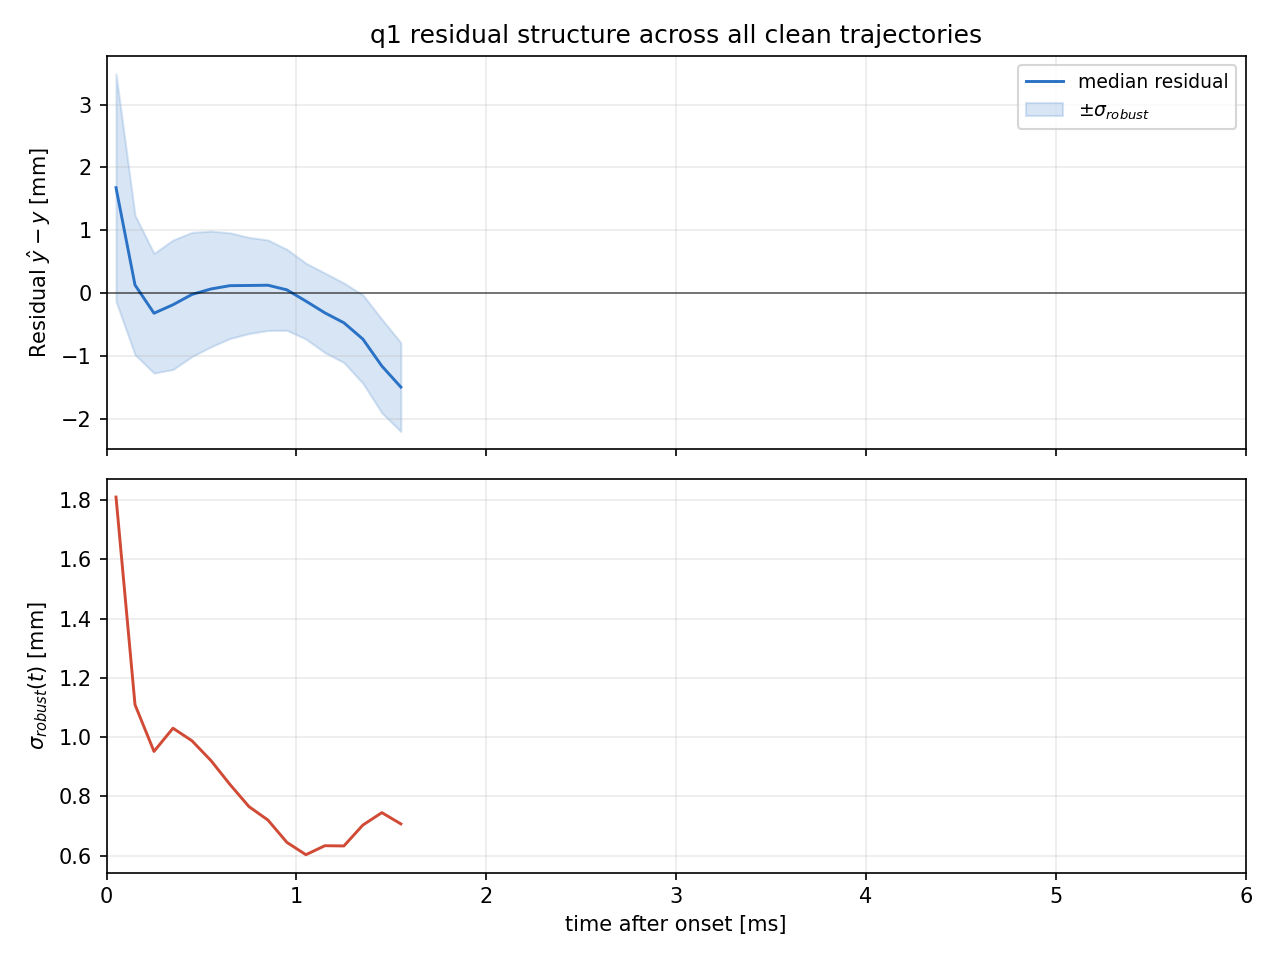
\includegraphics[width=0.92\linewidth]{images/fig_q1_residual_structure.png}
\caption{Residual structure of the q1 production fit aggregated across all \(24{,}316\) clean trajectories. Top panel: per-time-bin median residual with \(\pm\sigma_{\mathrm{robust}}\) shading. Bottom panel: robust standard deviation \(\sigma_{\mathrm{robust}}(t)=1.4826\,\mathrm{MAD}(t)\), exhibiting a U-shaped envelope -- onset-alignment noise inflates the first bin to \(\sim\SI{1.8}{mm}\), the central window reaches a minimum of \(\sim\SI{0.60}{mm}\) near \(t=\SI{1.0}{ms}\), and right-censoring of the surviving population inflates the late tail. The non-constant \(\sigma(t)\) motivates an input-dependent variance in the Stage-2 NLL loss.}
\label{fig:q1-residual-structure}
\end{figure}

\textbf{Parameter identifiability.} A third diagnostic computes asymptotic parameter standard errors and pairwise correlations from the trust-region Jacobian \(J\) returned by SciPy, \(\Sigma\approx (J^TJ)^{-1}\hat\sigma^2\). Across all clean fits the median pairwise correlations are \(\overline{\mathrm{corr}}(\log k_{1/4},\log s)\approx 0.76\), \(\overline{\mathrm{corr}}(\log k_{1/4},\log t_0)\approx 0.56\), and \(\overline{\mathrm{corr}}(\log t_0,\log s)\approx 0.21\). These are strong: the three q1 parameters are not independent physical handles but a coupled three-dimensional smoothing surface with substantial soft redundancy. This is the price the differentiable sigmoid gate pays compared to the rigid stage-by-stage breakpoint of Hiroyasu--Arai, and it also explains why the gating parameters scale poorly with operating conditions in the regression above: the data only constrains the surface as a whole, not each axis separately. In practice this shapes a downstream design choice: the surrogate models in Section~\ref{sec:mlp-curriculum-en} are trained to reproduce the full evaluated curve rather than the parameter triple itself, so the strong parameter coupling does not propagate into the trained network's input--output map.

\begin{figure}[t]
\centering
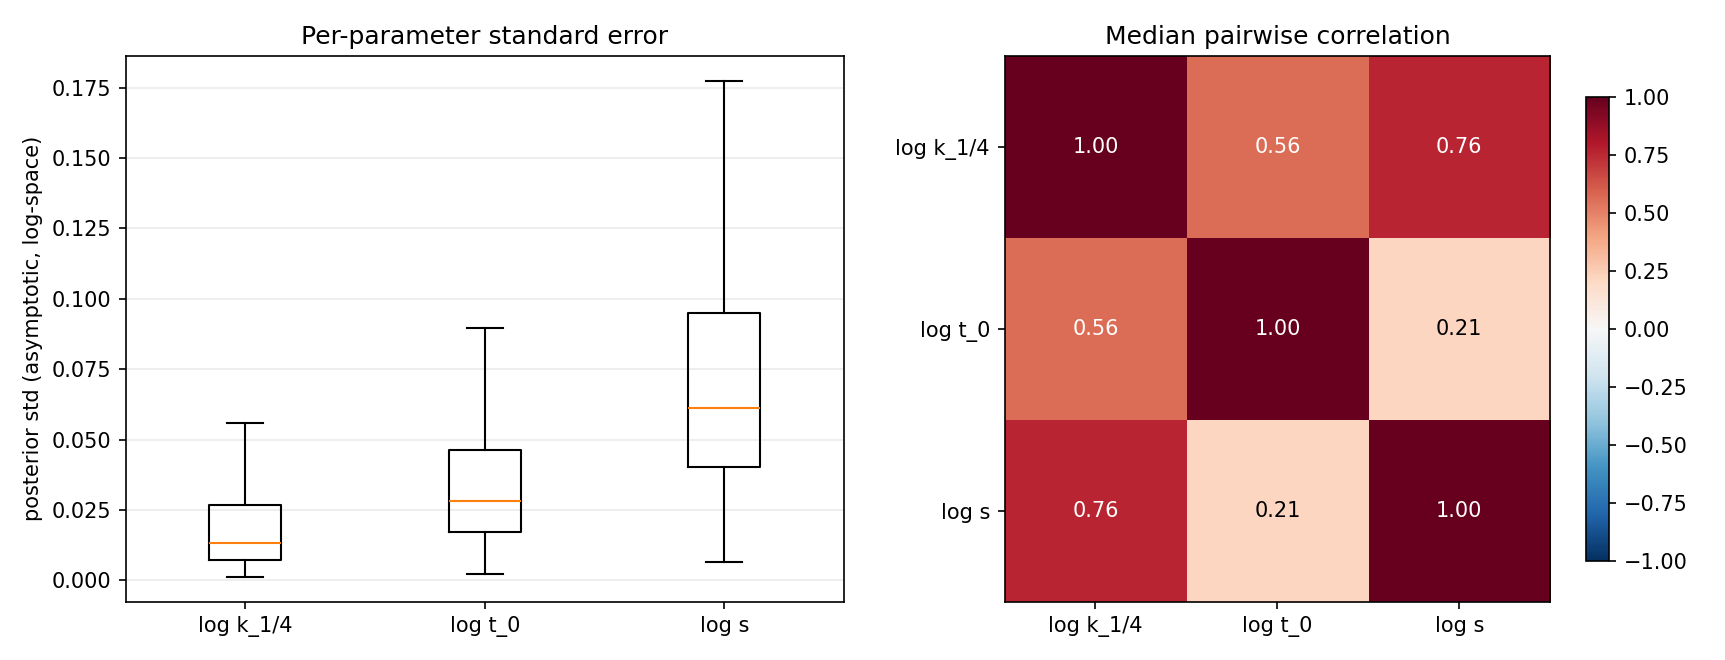
\includegraphics[width=0.96\linewidth]{images/fig_q1_identifiability.png}
\caption{Per-fit identifiability diagnostics for the q1 production model. Left: distribution of asymptotic standard errors of \(\log k_{1/4}\), \(\log t_0\), and \(\log s\) (clipped at the 99th percentile for readability). Right: median pairwise correlation matrix from \((J^TJ)^{-1}\); the off-diagonal entries \(\sim 0.56\) and \(\sim 0.76\) document the soft redundancy between branch amplitude and the sigmoid gate.}
\label{fig:q1-identifiability}
\end{figure}

Table~\ref{tab:q1-fit-diagnostics-summary} consolidates the headline statistics from the four diagnostics above so that they can be cross-referenced in later sections without re-deriving them. All numbers are exact values computed on the production archive.

\begin{table}[t]
\centering
\caption{Summary of q1 fit-quality diagnostics across the \(24{,}316\) accepted clean fits and \(703{,}592\) frame observations.}
\label{tab:q1-fit-diagnostics-summary}
\small
\begin{tabular}{p{0.30\linewidth} p{0.40\linewidth} p{0.22\linewidth}}
\toprule
\textbf{Diagnostic} & \textbf{Statistic} & \textbf{Value} \\
\midrule
Per-condition RMSE & median across (nozzle, $P_{\mathrm{inj}}$, $P_{\mathrm{ch}}$) bins & 0.62--1.80 mm \\
\midrule
Scaling regression for $k_{1/4}$ & exponents $(a,b,c)$ for $\Delta P^a \rho_a^b d_n^c$, with $R^2$ & $(0.52, -0.23, 0.26)$, $R^2=0.27$ \\
Hiroyasu--Arai post-breakup reference & $(\Delta P^{1/4}, \rho_a^{-1/4}, d_n^{1/2})$ & $(0.25, -0.25, 0.50)$ \\
\midrule
Residual median & central window $t\in[0.3, 1.0]\,\si{ms}$ & $|\,\cdot\,| < \SI{0.4}{mm}$ \\
Residual median & first bin ($t=\SI{0.05}{ms}$) & $\SI{+1.74}{mm}$ \\
Residual median & late tail ($t=\SI{1.55}{ms}$) & $\SI{-1.64}{mm}$ \\
Residual $\sigma_{\mathrm{robust}}$ & first bin ($t=\SI{0.05}{ms}$) & $\SI{1.80}{mm}$ \\
Residual $\sigma_{\mathrm{robust}}$ & minimum near $t=\SI{1.0}{ms}$ & $\SI{0.60}{mm}$ \\
Residual $\sigma_{\mathrm{robust}}$ & late tail ($t=\SI{1.55}{ms}$) & $\SI{0.71}{mm}$ \\
\midrule
Solver convergence & ftol-satisfied (count / fraction) & $24{,}228 / 24{,}316$ (99.6\%) \\
Solver convergence & timeouts (max\_nfev reached) & $0$ \\
Solver convergence & median nfev & $38$ \\
\midrule
Identifiability (median std) & $\log k_{1/4}$ \,/\, $\log t_0$ \,/\, $\log s$ & $0.013$ / $0.028$ / $0.061$ \\
Identifiability (median corr) & $\mathrm{corr}(\log k_{1/4}, \log s)$ & $0.76$ \\
Identifiability (median corr) & $\mathrm{corr}(\log k_{1/4}, \log t_0)$ & $0.56$ \\
Identifiability (median corr) & $\mathrm{corr}(\log t_0, \log s)$ & $0.21$ \\
\bottomrule
\end{tabular}
\end{table}

\subsubsection{Outlier masking and filter selection bias}

The stricter post-fit masking stage is also an important part of the engineering contribution. The robust outlier mask first forms a far-time penetration proxy by evaluating the fitted curve at \(t_{\mathrm{far}}=\SI{5}{ms}\). A row is retained only if that far-time value remains inside a broad physically plausible window and if the fit parameters pass basic sanity checks on \(t_0\), \(s\), point count, and fit cost. Robust grouped outlier scores are then computed using the median absolute deviation,
\[
z_{\mathrm{robust}}(x)=0.6745\,\frac{x-\operatorname{median}(x)}{\operatorname{MAD}(x)+\epsilon},
\qquad
\operatorname{MAD}(x)=\operatorname{median}\!\left(\lvert x-\operatorname{median}(x)\rvert\right),
\]
applied to \(t_0\), \(\log(1+\mathrm{RMSE})\), and \(\log(1+\mathrm{cost\_per\_point})\) within each file group. Rows with \(|z_{\mathrm{robust}}|>3\) on any of those diagnostics are marked as outliers and excluded from the clean archive.

This masking process introduces a deliberate engineering trade-off, and its dominant mechanism has shifted with upstream CV pipeline improvements. In earlier processing, uneven illumination or plume-to-plume occlusion sometimes caused the CV pipeline to misidentify background noise as the spray tip, producing physically impossible jumps that were then truncated into heavily shortened series by an explicit upper difference threshold; the \(n \ge 10\) frame floor and the \(t_0 < \SI{0.8}{ms}\) plausibility gate were primarily designed to intercept these degraded trajectories. After the CV enhancements, the vast majority of candidate series now pass the full masking pipeline (per-nozzle survival rates are reported in Figure~\ref{fig:filter-survival-cdf-nozzle} below). The sequences that do get flagged are typically \emph{longer} trajectories whose \(t_0\), RMSE, or \(\mathrm{cost\_per\_point}\) exceed the three-sigma robust threshold within their group, rather than short, noise-truncated series from CV misidentification. The masking logic therefore now functions more as a fit-quality gate than as a CV-artefact cleaner.

Consequently the filtering process introduces selection bias along two dimensions. The first is optical-quality bias: the surviving dataset favours well-illuminated, unobstructed, high-contrast plumes and does not represent genuine geometric asymmetries or late-stage signal fading. The second is injection-pattern regularity bias: q1 is structurally limited to monotonically increasing smooth penetration curves, and trajectories with non-monotone behaviour from bimodal injection or spray re-acceleration carry elevated within-group RMSE and are flagged by the robust z-score outlier gate. Per-nozzle flagging rates quantify the resulting coverage gap: on the CDF source, Nozzle~3 is flagged at 11.9\%, roughly twice the rate of Nozzle~4 and Nozzle~6 (both 5.9\%), consistent with the spray re-acceleration events observed for Nozzle~3 in the Stage-3 diagnostics. Stage-1 and Stage-2 therefore inherit both biases together: their training set is skewed toward optically ideal plumes and toward trajectories whose injection pattern is regular enough for the q1 monotone form to represent adequately.

Figure~\ref{fig:filter-survival-cdf-nozzle} shows the CDF penetration q1 filter survival rate per nozzle, summarising total series, cleaned series, and pass ratio. The purpose of this figure is not to argue that the filter is unbiased; it is to make the coverage of that bias explicit. After regenerating the report against the restored PC archive, the nine-nozzle campaign spans a CDF penetration survival-rate band of \(88.1\%\)--\(94.1\%\). The restored Nozzle0 archive contributes \(\num{15475}\) candidate CDF penetration series, of which \(\num{14274}\) survive the clean-fit filter (\(92.2\%\)), so it is part of the reported coverage. Because no nozzle is nearly fully rejected or nearly fully retained, Stage~2 can be interpreted as a clean-plume teacher over the restored archive, while still inheriting the location and late-stage selection bias made explicit here.

\begin{figure}[t]
\centering
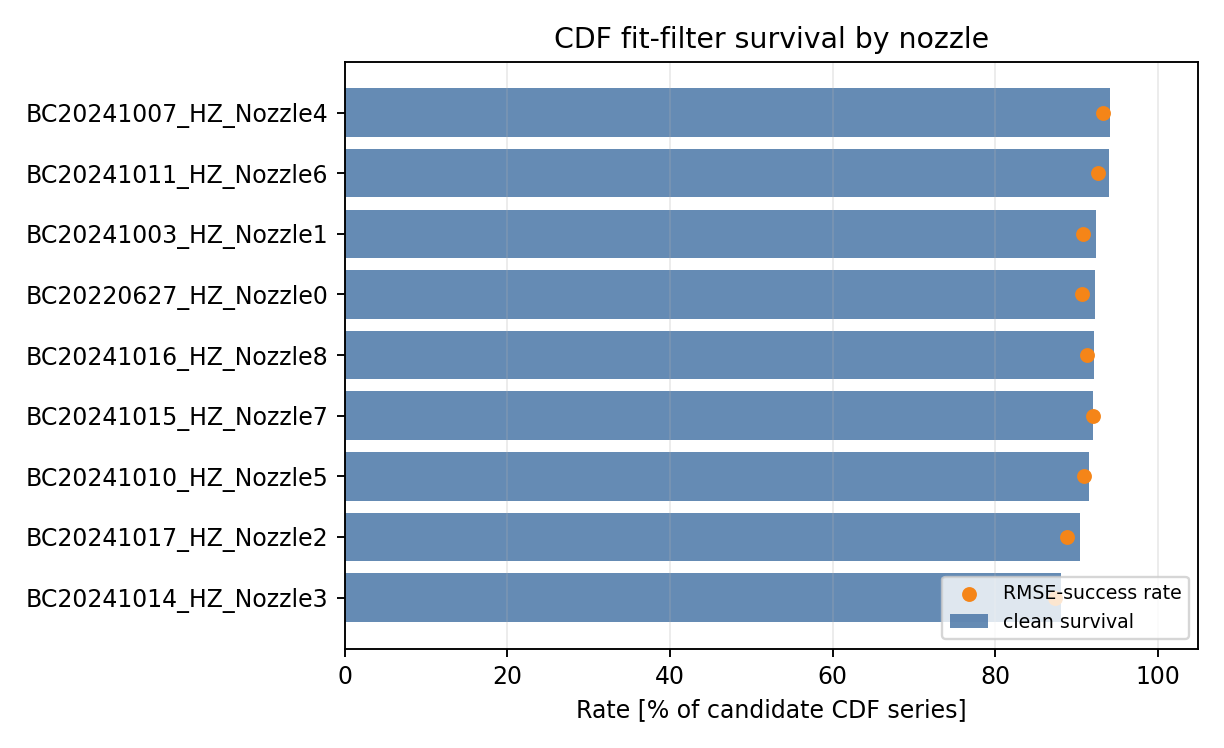
\includegraphics[width=0.88\linewidth]{images/filter_survival_cdf_by_nozzle.png}
\caption{CDF penetration q1 filter survival rate regenerated from the restored PC archive. The figure reports the total candidate series count, cleaned series count, and pass ratio for all nine nozzle families, including Nozzle0.}
\label{fig:filter-survival-cdf-nozzle}
\end{figure}

\begin{table}[t]
\centering
\footnotesize
\input{../generated/current/data_attrition_tex.tex}
\caption{Trajectory attrition with a common raw-trajectory denominator. This generated table avoids multiplying percentages measured on different populations; each gate is reported as an absolute count against the raw CDF penetration plume inventory.}
\label{tab:data-attrition-generated}
\end{table}

The trade-off is deliberate but limited. By excluding ambiguous data, the pipeline gives Stage~2 a clean teacher target that is less exposed to optical vanishing effects, background reflections, and incorrect hydraulic delay alignments. Stage~3 then recombines this clean prior with the raw, unfiltered CDF penetration data: it trusts raw observations in high-confidence bins and falls back to the Stage~2 teacher where coverage collapses. The result is a controlled interpolation between early-time raw-signal fidelity and late-time physical consistency.

That design does not remove the selection bias introduced by filtering. The teacher's late-time prior remains conditioned on well-illuminated, unobstructed plumes; when Stage~3 defers to it, the output should be read as a clean-plume continuation rather than as a debiased ensemble over all nozzle geometries.

\textbf{Overall assessment of the q1 reduced-order surrogate.} The combined evidence positions \(S(t)=\sigma((t-t_0)/s)\,k_{1/4}\,t^{1/4}\) as a numerically robust reduced-order trajectory surrogate rather than a new closed-form penetration law. The kinematic exponent \(t^{1/4}\) inherits the regime-change shape used by Hiroyasu and Arai \cite{HiroyasuArai1990} and the post-EOI extensions of Zhou et al.\ \cite{ZhouLiLaiWei2019,ZhouLiYi2021}, while the sigmoid gate replaces their hard breakpoint with a differentiable transition --- the structural prerequisite for using fitted curves as targets in a downstream neural surrogate. The empirical \(k_{1/4}\) scaling matches the Hiroyasu--Arai free-jet predictions in \(\rho_a\) and \(d_n\) closely; the steeper \(\Delta P\) exponent is reported as an empirical observation rather than a confirmed regime shift. The four-parameter blend collapses to \(k_{\mathrm{sqrt}}\!\approx\!0\) in \(99.8\%\) of fits, so the data itself selects the quarter-root branch, and the central-window robust spread of \(\sim\SI{0.60}{mm}\) sits near the optical noise floor of the imaging chain.

Two limitations are worth stating explicitly. First, the three q1 parameters are not independent physical handles --- the soft redundancy between branch amplitude and the sigmoid gate makes \((k_{1/4}, t_0, s)\) a coupled smoothing surface rather than three separate coefficients. Second, the dimensional group \((\Delta P, \rho_a, d_n)\) explains only \(R^2\!\approx\!0.27\) of the log-space variance in \(k_{1/4}\). Both are absorbed by the surrogate-stack design: Stage~1--3 train networks to reproduce the evaluated curve \(\hat S(\cdot)\) rather than the parameter triple, so the coupling does not propagate into the trained input--output map; and the unexplained trajectory-level variance is precisely the heteroscedastic residual that the Stage-2 NLL and the Stage-3 distillation are introduced to handle. The principal use range \(0\)--\(\SI{1.5}{ms}\) sits inside the data-dominated zone of the q1 fit, while the boundary inflations and parameter coupling primarily affect the \(>\SI{2}{ms}\) far-field, where Stage-3 already defers to the teacher's conservative envelope.

In the population terminology of Section~\ref{sec:three-derived-populations-en}, the q1 fit defines Dataset~\#3. This is the smooth archive from which the Stage~2 teacher is learned, including its useful clean-plume prior and its filtering bias. Stage~3 later reintroduces Dataset~\#1 in reliable coverage bins to recover raw early-time behaviour without trusting the right-censored tail as if it were fully observed.

\subsection{Physics-guided feature engineering}
\label{sec:feature-engineering-en}

Before the engineered-feature architecture was finalised, an earlier nine-feature MLP was trained with direct pressure and diameter inputs and revealed a structural pathology. Nozzle diameter has only six levels in the dataset and is not uniformly available across pressure combinations---all six diameter levels appear only on the family $(P_{\mathrm{inj}}=\SI{2000}{bar},\;P_{\mathrm{cb}}=4,\;P_{\mathrm{ch}}\in\{5,10,15\}\,\si{bar})$---and injection pressure has only four levels. Figure~\ref{fig:sparse-support-topology} makes this discrete sampling grid explicit: most cells of the (chamber-pressure, injection-pressure, diameter) lattice contain zero or one observation, and the full six-diameter coverage exists only along a single pressure family.

\begin{figure}[t]
\centering
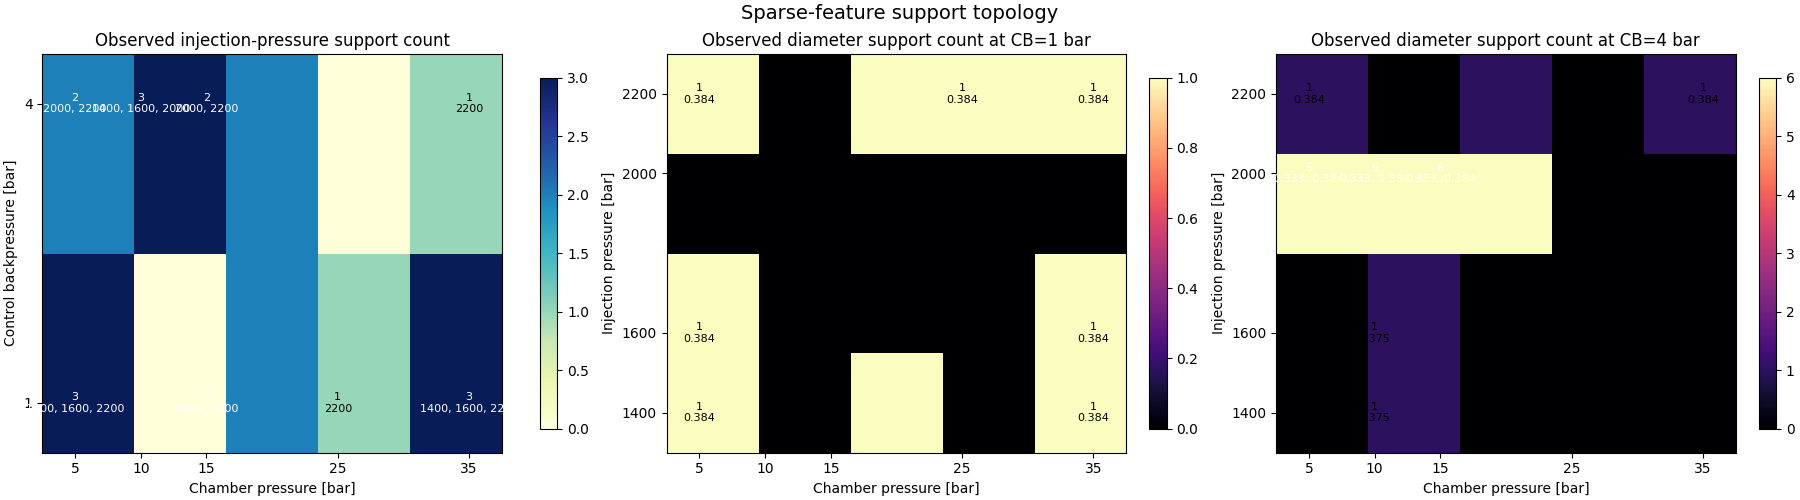
\includegraphics[width=0.96\linewidth]{images/fig_sparse_support_topology.png}
\caption{Sparse-feature support topology of the training matrix. Left: observed injection-pressure support count over the (chamber pressure, control back-pressure) plane, with the available levels annotated per cell. Centre and right: observed nozzle-diameter support count at $\mathrm{CB}=\SI{1}{bar}$ and $\mathrm{CB}=\SI{4}{bar}$ over the (chamber pressure, injection pressure) plane. Most cells contain zero or one diameter level; the full six-level diameter coverage appears only on the narrow family $(P_{\mathrm{inj}}=\SI{2000}{bar},\;\mathrm{CB}=4,\;P_{\mathrm{ch}}\in\{5,10,15\}\,\si{bar})$.}
\label{fig:sparse-support-topology}
\end{figure}

Because a smooth MLP treats these as continuous inputs, it produces derivative structure along the diameter and pressure axes that the data do not constrain. Figure~\ref{fig:sparse-diameter-interpolants} shows the consequence on dense diameter sweeps at $t=\SI{0.85}{ms}$: between adjacent observed levels the predicted-mean curve oscillates through five to six gradient sign changes per slice, and the autograd gradient peaks near $\sim\!\SI{4e4}{}$ over support spans of order \SI{0.05}{mm}, i.e.~curvature norms of order~$10^7$. The same diagnostic on injection pressure shows non-monotone, unsupported extrapolation on thinly supported slices. The underlying problem is structural---a smooth MLP being asked to learn a continuous law from an effectively discrete grid---so adding regularisation would only suppress instability at the cost of useful capacity. The revised architecture therefore addresses this at the source.

\begin{figure}[t]
\centering
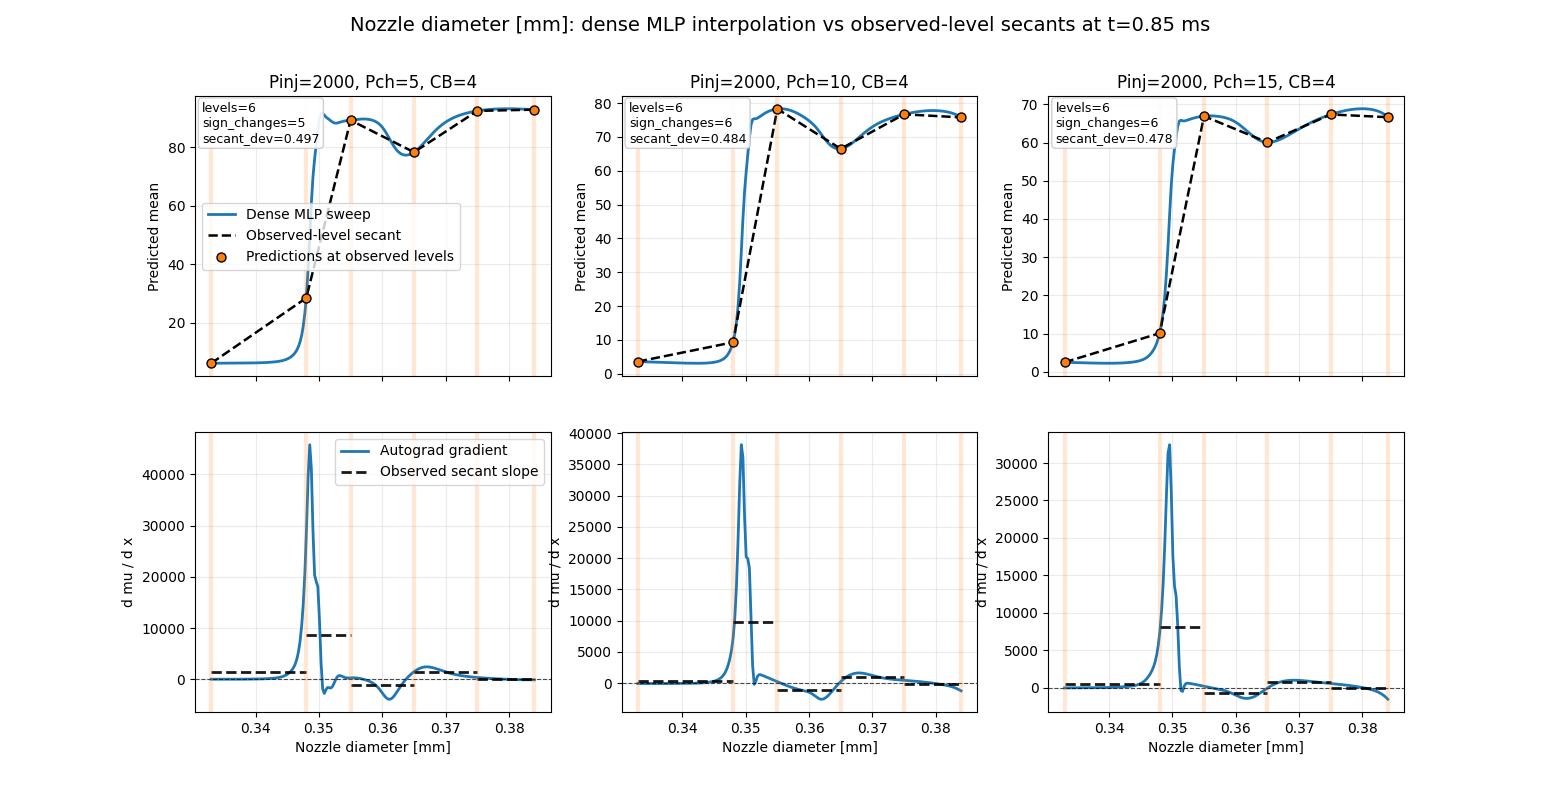
\includegraphics[width=0.98\linewidth]{images/fig_sparse_diameter_interpolants.png}
\caption{Dense MLP interpolation along the nozzle-diameter axis at $t=\SI{0.85}{ms}$ for three operating points (columns), under the direct-feature baseline. Top row: predicted mean (blue) compared with the observed-level secant (dashed black) through the six diameter levels (orange). Bottom row: autograd gradient $\partial\mu/\partial d_n$ (blue) versus the observed secant slopes (dashed black). The MLP produces five to six gradient sign changes per slice and gradient spikes of order $10^4$ over support spans of \SI{0.05}{mm}, none of which are constrained by the data.}
\label{fig:sparse-diameter-interpolants}
\end{figure}

The revised surrogate replaces the four weakly supported pressure and diameter inputs with a single hard scaling group. The Hiroyasu--Arai post-breakup branch \cite{HiroyasuArai1990} provides the dimensional motivation:
\[
S(t)\;\propto\;K_p\!\left(\frac{\Delta P}{\rho_a}\right)^{1/4}d_n^{1/2}\,t^{1/2},
\]
where the H--A exponent assigns $\Delta P^{1/4}$ to the pressure-ratio group. The empirical scaling regression reported above, however, finds a $\Delta P$ exponent of approximately $0.52$ across the mid-injection window---roughly twice the H--A value---so the amplitude scale is updated to reflect the data:
\[
A\;=\;\Delta P^{0.5}\cdot\rho_a^{-0.25}\cdot d_n^{0.5},
\]
computed from the canonical feature table derived from the test-matrix JSON files. This form retains the H--A $\rho_a^{-1/4}$ and $d_n^{1/2}$ exponents, where the empirical regression shows good agreement, while adopting $\Delta P^{0.5}$ in place of the H--A $\Delta P^{1/4}$. For Nozzle1--Nozzle8 the chamber density is taken directly from the recorded ambient gas density; for Nozzle0, which records only the ambient chamber pressure, $\rho_a$ is reconstructed from the linear law $\rho_a=\SI{5}{kg/m^3}\times P_{\mathrm{ch}}/\SI{4.42}{bar}$ calibrated against the Nozzle1--8 data.

The exponent change should not be read as a rejection of the Hiroyasu--Arai asymptote. A time-windowed log--log regression on the observed CDF penetration shows a transition: the \(\Delta P\) exponent is close to the Bernoulli/orifice value near the dense mid-trajectory window (\(a\approx0.48\)--\(0.58\) around \(t=\SI{0.4}{ms}\)--\(\SI{0.6}{ms}\)), and approaches the H--A value of \(0.25\) closer to \(t=\SI{1.0}{ms}\). The representative training mass is therefore not dominated by a purely late entrainment asymptote; it still carries a strong transitional momentum imprint. The selected \(\Delta P^{0.5}\) scale is an empirical compromise for the present short-pilot archive, while \(\Delta P^{0.25}\) remains the appropriate late-time physical reference.

A pre-training collapse check makes this assumption falsifiable before any MLP weights are updated. The diagnostic reconstructs trajectories, divides each by its own \(A\), and measures whether the sparse pressure/diameter axes still explain the scaled target. Comparing \(\Delta P^{0.25}\) and \(\Delta P^{0.5}\), both pass the weak criterion that post-\(\SI{0.5}{ms}\) scaled spreads remain below the unscaled spread, but \(\Delta P^{0.5}\) collapses the archive much more strongly: the median post-\(\SI{0.5}{ms}\) collapse ratio falls from \(0.378\) to \(0.057\), and the scaled/physical sparse-feature \(R^2\) ratio falls from \(0.130\) to \(0.055\). This is the pre-training counterpart to the LONO feature ablation below.

In the first design iteration, all four sparse inputs are folded entirely into $A$, producing a five-feature scaling-only baseline
\[
[\,t_{\mathrm{norm}},\;\theta_{\mathrm{tilt},z},\;n_{\mathrm{plumes},z},\;t_{i,z},\;P_{\mathrm{cb},z}\,],
\]
where $A$ serves only as a target divisor and does not enter the network. The training target is reparameterised to the non-dimensional penetration $\hat{S}(t)=S(t)/A$; the network predicts $\hat{\mu}$ and $\log\hat{\sigma}^2$, and physical predictions are recovered at inference as $\mu_S=A\,\hat{\mu}$ and $\sigma_S=A\,\hat{\sigma}$. This baseline achieved a Stage-1 test MAE of \SI{8.05}{mm} and a Stage-2 test MAE of \SI{9.28}{mm}.

Folding $P_{\mathrm{inj}}$ and $P_{\mathrm{ch}}$ entirely into $A$, however, removes their individual explanatory power beyond what the fixed $\Delta P^{0.5}$ exponent captures. The regression also estimates a non-zero chamber-pressure coefficient at fixed $\Delta P$ (approximately $-0.21$ to $-0.27$ across the mid-injection window), so $P_{\mathrm{inj}}$ and $P_{\mathrm{ch}}$ carry independent structure that cannot be fully collapsed into $\Delta P$ alone. The global $\Delta P^{0.5}$ exponent is itself a mean-field approximation, and any local residual nonlinearity across the condition space is left outside the network's reach when $P_{\mathrm{inj}}$ and $P_{\mathrm{ch}}$ are absent. Nozzle diameter $d_n$ is a different case: it has only six discrete levels in the dataset and suffers severe confounding in the condition matrix (Figure~\ref{fig:sparse-support-topology}), making it an unreliable continuous input even if reintroduced. It therefore remains inside $A$, with the H--A prior carrying its effect.

On this basis, the final design adopts a seven-feature scaling-plus-residual-pressure form
\[
[\,t_{\mathrm{norm}},\;\theta_{\mathrm{tilt},z},\;n_{\mathrm{plumes},z},\;t_{i,z},\;P_{\mathrm{cb},z},\;\log P_{\mathrm{inj},z},\;\log P_{\mathrm{ch},z}\,],
\]
where $A$ continues to absorb the dominant diameter and dimensional pressure dependence, while $\log P_{\mathrm{inj}}$ and $\log P_{\mathrm{ch}}$ are fed as separate inputs so the network can learn residual pressure structure beyond the H--A fixed exponents. Compared with the five-feature baseline, Stage-1 test MAE falls from \SI{8.05}{mm} to \SI{2.91}{mm} and Stage-2 test MAE falls from \SI{9.28}{mm} to \SI{5.63}{mm}, confirming that the residual pressure features supply information that the fixed H--A exponents obscure.

Before any optimisation, a scaling-validation routine tests the scaling assumption on the actual dataset: each trajectory is divided by its own $A$, and a linear-regression $R^2$ of $\hat{S}(t)$ on the sparse features is computed. In the seven-feature production run the check passed with the sparse-feature $R^2$ dropping from $0.32$ on the physical target $S$ to $0.016$ on the scaled target $\hat{S}$, so $A$ does account for the dominant diameter and pressure variation, leaving the network to learn residual structure on the $\log P_{\mathrm{inj}}$ and $\log P_{\mathrm{ch}}$ axes. If the check fails, training aborts by default, so the physical prior is falsifiable rather than merely asserted: the empirically calibrated exponents in $A = \Delta P^{0.5}\cdot\rho_a^{-0.25}\cdot d_n^{0.5}$ carry an empirically checkable prediction that the training protocol confirms or rejects before any weights are updated.

Stage~1 and Stage~2 also share a group-aware data split: whole operating-condition groups — defined by nozzle identity, injection pressure, chamber pressure, and injection duration — are assigned together to train, validation, or test, preventing leakage between curves that share an operating point. Without this constraint, a random trajectory-level split would let the network interpolate between near-identical curves from the same operating condition seen during training, and the held-out error would reflect intra-condition smoothness rather than generalisation across the condition space. The group assignment is therefore the structural guarantee that the reported test metrics describe interpolation across distinct operating conditions rather than memorisation within them. Stage~2 warm-starts from the Stage-1 engineered run directory and reuses its scaler state, so variant choice and $A$-scaling are consistent across both stages.

\subsubsection{Cross-population scaling verification on Dataset \#2}
\label{sec:pointlevel-scaling-verification}

A complementary and more direct verification of the scaling group $A$ is carried out on Dataset~\#2 from Section~\ref{sec:three-derived-populations-en}, rather than on the q1-fitted archive that motivated the first exponent estimate. The point-level dataset is constructed by the right-censoring point-table tool (\texttt{build\_cdf\_right\_censoring\_point\_table}). For each of the \num{592} operating-condition groups the tool expands the \texttt{series\_wide\_clean} wide-format table into a long-format record of individual $(t,\,S)$ observations, bins them into $\Delta t=\SI{0.1}{ms}$ intervals over $[0,\SI{5}{ms}]$, and determines a per-condition censoring threshold jointly from two criteria: (i)~the smoothed per-bin trajectory count falling below a fixed fraction of its within-condition peak (density-drop criterion), and (ii)~the per-bin $p_{95}$ penetration reaching $95\%$ of the estimated field-of-view cap (FOV-saturation criterion). All observations at or beyond the first bin satisfying either criterion are labelled right-censored and excluded, leaving $N_{\mathrm{unc}}=\num{506634}$ uncensored points.

\textbf{Per-condition temporal balance.}
A direct concern for any regression on time-indexed penetration observations is that trajectories surviving to late time bins are a progressively self-selected subset of the population — potentially biasing the sample towards slow or wall-bounded plumes. The per-condition truncation eliminates this concern. Before applying the right-censoring label, the median coefficient of variation of the per-bin trajectory count across time is $\mathrm{CV}_{\mathrm{raw}}=0.52$, reflecting the progressive dropout as trajectories hit the field-of-view boundary. After truncating each condition at its censoring threshold, the median per-condition CV falls to $\num{0.052}$ (interquartile range $[0.033,\;0.082]$), and the median ratio of the minimum to the mean bin count within a condition is $0.92$. Within each surviving window, point counts are therefore approximately uniform in time: the censoring removes the trajectory-depleted tail rather than reweighting it, and each retained time bin contributes statistically comparable evidence to a downstream regression.

\textbf{Log-log scaling regression.}
The ordinary-least-squares regression
\[
  \log S = a\log\Delta P + b\log P_{\mathrm{ch}} + c\log d_n + \mathrm{const}
\]
is fitted independently at each \SI{0.1}{ms} bin, where $\Delta P = P_{\mathrm{inj}}-P_{\mathrm{ch}}$ and $P_{\mathrm{ch}}$ is used as a proportional proxy for the ambient density $\rho_a$ (valid for ideal-gas conditions at constant temperature). Table~\ref{tab:loglog-regression-uncensored} reports the results in the informative mid-trajectory window $t\in[0.30,\;0.70]\,\si{ms}$, where both point counts and signal strength are high.

\begin{table}[t]
\centering
\footnotesize
\begin{tabular}{@{}crrrrr@{}}
\toprule
$t$ [ms] & $a_{\Delta P}$ & $b_{P_{\mathrm{ch}}}$ & $c_{d_n}$ & $R^2$ & $N$ \\
\midrule
0.30 & $0.682$ & $-0.232$ & $6.015$ & $0.351$ & 72\,547 \\
0.40 & $0.523$ & $-0.247$ & $4.461$ & $0.392$ & 63\,414 \\
0.50 & $0.472$ & $-0.229$ & $3.064$ & $0.398$ & 56\,117 \\
0.60 & $0.521$ & $-0.189$ & $2.178$ & $0.418$ & 46\,466 \\
0.70 & $0.447$ & $-0.153$ & $1.693$ & $0.354$ & 38\,291 \\
\midrule
H--A reference & $0.25$ & $-0.25$ & $0.50$ & --- & --- \\
\bottomrule
\end{tabular}
\caption{Per-bin log-log regression of uncensored CDF penetration against $(\Delta P,\,P_{\mathrm{ch}},\,d_n)$ on the \num{506634} right-censored point dataset. Each row is an independent OLS regression on all points in the $\pm\SI{0.05}{ms}$ window around the stated bin centre. The Hiroyasu--Arai post-breakup reference exponents are listed for comparison. The $c_{d_n}$ column is unreliable for the structural reasons explained in the text.}
\label{tab:loglog-regression-uncensored}
\end{table}

The injection-pressure exponent $a$ stabilises at $0.47$--$0.52$ in the $0.40$--$0.60\,\si{ms}$ window, close to the Bernoulli value of $0.5$ and to the earlier $k_{1/4}$ regression ($a\approx0.52$). The chamber-pressure exponent $b$ stabilises at $-0.23$ to $-0.25$, in close agreement with the Hiroyasu--Arai prediction of $-0.25$ and the $k_{1/4}$ estimate ($b\approx-0.23$). Both exponents are stable across the two datasets (the compressed $k_{1/4}$ parameter and the raw point observations), so the $\Delta P^{0.5}\cdot\rho_a^{-0.25}$ components of $A$ are not artefacts of the fitting procedure.

\textbf{Diameter exponent and the H--A prior.}
The $c_{d_n}$ column in Table~\ref{tab:loglog-regression-uncensored} is large and varies from $1.7$ to $6.0$; these values have no physical interpretation. Two structural reasons make the diameter exponent unidentifiable from this dataset. First, the six nozzle-hole diameters span only $0.333$--$\SI{0.384}{mm}$ (ratio $1.15$, log-leverage $0.14$), roughly three times smaller than the log-leverage available from the injection-pressure range ($0.45$). Second, pressure and diameter are not independently varied across the design matrix: the full six-diameter coverage appears only within a single injection-pressure family ($P_{\mathrm{inj}}=\SI{2000}{bar}$, $P_{\mathrm{cb}}=\SI{4}{bar}$), and within that family the nozzle families differ not only in hole diameter but also in hole count and umbrella angle. A controlled check within this matched-pressure family --- regressing the per-condition median penetration against $\log d_n$ at fixed $\Delta P$ and $P_{\mathrm{ch}}$ --- yields $c_{d_n}\approx 0$ with $R^2<0.01$ throughout the mid-trajectory window, confirming that the causal diameter effect cannot be isolated from geometry confounders in this dataset. The $d_n^{0.5}$ term in $A$ is therefore retained as the Hiroyasu--Arai physically motivated prior; the two components that are empirically supported, $\Delta P^{0.5}$ and $\rho_a^{-0.25}$, are confirmed by both the $k_{1/4}$ regression and the present point-level check on the right-censored dataset.

\subsubsection{LONO ablation of the engineered-feature design}
\label{sec:stage1-lono-ablation}

The single-split improvement reported earlier in this subsection (Stage-1 test MAE \SI{8.05}{mm}\(\to\)\SI{2.91}{mm}) confirms that the seven-feature design outperforms the scaling-only baseline within the same group-aware split. A more demanding test is whether the design choices generalise to nozzle families never seen during training. A dedicated leave-one-nozzle-out (LONO) ablation evaluates all nine variants of the engineered-feature design on a five-fold split in which each of Nozzle0, Nozzle1, Nozzle2, Nozzle4, and Nozzle5 is held out in turn while the remaining four families form the training pool. Every cell of the ablation uses the same deterministic Stage-1 MSE objective described in Section~\ref{sec:mlp-curriculum-en}, the same network architecture and optimiser, and a single fixed seed (42), so the only varying axis is the feature configuration.

The nine variants vary three orthogonal design axes: the amplitude exponent (\(\alpha=0.25\) vs.\ \(\alpha=0.5\) in \(A=\Delta P^{\alpha}\rho_a^{-0.25}d_n^{0.5}\)), the presence of log-pressure residuals (\(\log P_{\mathrm{inj},z}\), \(\log P_{\mathrm{ch},z}\)), and the presence of \(d_n\) as a standalone input. A legacy nine-feature configuration that pre-dates the amplitude scaling (\texttt{legacy\_9\_no\_scale}; raw \(\log P_{\mathrm{inj}}\), \(\log P_{\mathrm{ch}}\), \(\log\Delta P\), and \(d_n\) all fed directly to the network with target \(S\) in millimetres) is included for reference. Table~\ref{tab:stage1-lono-ablation-summary} reports the mean physical MAE across the five folds, and Table~\ref{tab:stage1-lono-ablation-per-fold} breaks the results down per fold.

Three patterns are consistent across the design axes:
\begin{enumerate}
\item \textbf{The exponent \(\alpha=0.5\) beats the Hiroyasu--Arai \(\alpha=0.25\) at every residual-feature level.} Pairing \texttt{a\_dp050} variants against their \texttt{a\_dp025} counterparts gives \SI{7.46}{mm} vs.\ \SI{8.22}{mm} (with pressures), \SI{8.27}{mm} vs.\ \SI{9.83}{mm} (no residuals), \SI{12.06}{mm} vs.\ \SI{13.41}{mm} (with diameter), and \SI{14.26}{mm} vs.\ \SI{14.48}{mm} (with both). The data-supported exponent absorbs more physical variance into \(A\) than the H--A value, leaving less unexplained residual for the network --- the LONO counterpart of the point-level scaling regression in Table~\ref{tab:loglog-regression-uncensored}.
\item \textbf{Adding the log-pressure residuals gives a small but consistent LONO gain over the pure scaling-only variant.} For \(\alpha=0.5\) the mean MAE falls from \SI{8.27}{mm} to \SI{7.46}{mm}; for \(\alpha=0.25\) it falls from \SI{9.83}{mm} to \SI{8.22}{mm}. The gain is consistent with the non-zero chamber-pressure coefficient at fixed \(\Delta P\) reported earlier in this subsection: \(P_{\mathrm{inj}}\) and \(P_{\mathrm{ch}}\) carry residual structure beyond what the fixed \(\Delta P^{0.5}\) exponent captures.
\item \textbf{Re-introducing \(d_n\) as a standalone input is strictly harmful under LONO.} Adding \texttt{diameter\_mm\_z} to any amplitude-scaled variant increases the mean MAE by \SI{4}{}--\SI{6}{mm}: \texttt{a\_dp050\_plus\_diameter} reaches \SI{12.06}{mm}, and the \texttt{plus\_pressures\_diameter} variants are the worst performers in the table (\(>\SI{14}{mm}\)), even slightly below the legacy nine-feature baseline. Because \(d_n\) is already encoded in \(A\) and has only six discrete levels with severe confounding (Figure~\ref{fig:sparse-support-topology}), the redundant channel lets the network memorise nozzle identity rather than generalise across families. This is the strongest direct evidence supporting the decision to leave \(d_n\) inside \(A\) rather than re-expose it to the network.
\end{enumerate}

The production variant \texttt{a\_dp050\_plus\_pressures} obtains the lowest mean LONO MAE (\SI{7.46}{mm}) and the most consistent per-fold performance of all nine configurations tested, with no single-fold result exceeding \SI{19}{mm}; the legacy nine-feature baseline reaches \SI{27.29}{mm} on its worst fold (Nozzle4). Even the simplest amplitude-scaled variant (\texttt{a\_dp025}) improves on the legacy baseline by \(\sim\!\SI{4.6}{mm}\) on the LONO mean, confirming that the amplitude-scaling step is the load-bearing element of the engineered-feature design. The Nozzle0 fold dominates the mean because it contributes 1{,}038 file-level sample groups --- roughly five times more than any other fold --- and is the only first-generation nozzle family with a substantially different geometric design from Nozzle1--Nozzle8, so its out-of-nozzle gap is inherently larger; even on this fold the production variant remains within \(\SI{0.21}{mm}\) of the best amplitude-scaled variant without standalone \(d_n\).

\begin{table}[t]
\centering
\footnotesize
\begin{tabular}{@{}rL{0.42\linewidth}rr@{}}
\toprule
Rank & Variant & MAE mean [mm] & MAE std [mm] \\
\midrule
1 & \texttt{a\_dp050\_plus\_pressures} (production) & \textbf{7.46} & 6.52 \\
2 & \texttt{a\_dp025\_plus\_pressures} & 8.22 & 8.55 \\
3 & \texttt{a\_dp050} & 8.27 & 6.08 \\
4 & \texttt{a\_dp025} & 9.83 & 7.59 \\
\midrule
5 & \texttt{a\_dp050\_plus\_diameter} & 12.06 & 7.67 \\
6 & \texttt{a\_dp025\_plus\_diameter} & 13.41 & 7.60 \\
7 & \texttt{a\_dp050\_plus\_pressures\_diameter} & 14.26 & 9.69 \\
8 & \texttt{legacy\_9\_no\_scale} & 14.42 & 9.43 \\
9 & \texttt{a\_dp025\_plus\_pressures\_diameter} & 14.48 & 10.21 \\
\bottomrule
\end{tabular}
\caption{LONO ablation of the engineered-feature design. Each row is the mean and standard deviation of the held-out physical MAE across the five leave-one-nozzle-out folds (held-out families: Nozzle0, Nozzle1, Nozzle2, Nozzle4, Nozzle5). All amplitude-scaled variants use \(A=\Delta P^{\alpha}\rho_a^{-0.25}d_n^{0.5}\) as a target divisor; the legacy variant fits \(S\) in millimetres with no amplitude scaling. The top block (\(A\)-scaled without standalone \(d_n\)) outperforms every variant that either re-exposes \(d_n\) or omits the amplitude scaling. The Stage-1 MSE in dimensionless space is not directly comparable between \(\alpha=0.25\) and \(\alpha=0.5\) because the target divisor differs; the physical MAE in millimetres is the correct cross-variant metric.}
\label{tab:stage1-lono-ablation-summary}
\end{table}

\begin{table}[t]
\centering
\footnotesize
\setlength{\tabcolsep}{4pt}
\begin{tabular}{@{}L{0.34\linewidth}rrrrr|r@{}}
\toprule
Variant & Nozzle0 & Nozzle1 & Nozzle4 & Nozzle5 & Nozzle2 & Mean \\
& \footnotesize(1038) & \footnotesize(81) & \footnotesize(81) & \footnotesize(81) & \footnotesize(195) & \\
\midrule
\texttt{a\_dp050\_plus\_pressures} & 18.95 & 4.65 & 5.47 & 2.76 & 5.48 & \textbf{7.46} \\
\texttt{a\_dp025\_plus\_pressures} & 23.42 & 4.35 & 5.18 & 2.86 & 5.27 & 8.22 \\
\texttt{a\_dp050} & 18.74 & 3.32 & 5.37 & 7.93 & 5.98 & 8.27 \\
\texttt{a\_dp025} & 22.59 & 3.17 & 5.14 & 8.62 & 9.64 & 9.83 \\
\midrule
\texttt{a\_dp050\_plus\_diameter} & 15.01 & 11.71 & 23.39 & 4.31 & 5.87 & 12.06 \\
\texttt{a\_dp025\_plus\_diameter} & 20.90 & 14.16 & 20.67 & 4.74 & 6.60 & 13.41 \\
\texttt{a\_dp050\_plus\_pressures\_diameter} & 22.34 & 11.79 & 26.14 & 3.23 & 7.80 & 14.26 \\
\texttt{legacy\_9\_no\_scale} & 19.81 & 12.41 & 27.29 & 2.75 & 9.83 & 14.42 \\
\texttt{a\_dp025\_plus\_pressures\_diameter} & 22.32 & 11.68 & 27.39 & 2.34 & 8.67 & 14.48 \\
\bottomrule
\end{tabular}
\caption{Per-fold LONO physical MAE for the nine engineered-feature variants. All values are in millimetres on the held-out nozzle test split. Numbers in parentheses are the file-level sample-group counts contributed by each held-out fold. Top block: \(A\)-scaled variants without standalone \(d_n\); bottom block: variants that either re-expose \(d_n\) or omit the amplitude scaling. The production variant \texttt{a\_dp050\_plus\_pressures} attains either the best or near-best result on every fold and is the only configuration whose worst-fold MAE remains below \SI{19}{mm}.}
\label{tab:stage1-lono-ablation-per-fold}
\end{table}

The single-split improvement reported earlier in this subsection and the LONO ablation reported here are mutually consistent: amplitude scaling is the load-bearing element, the log-pressure residuals supply a modest further gain, and the diameter remains absorbed into \(A\) rather than re-exposed. The numerical values differ because the LONO protocol holds out an entire nozzle family rather than a stratified random subset; the LONO mean MAE (\SI{7.46}{mm}) sits above the in-domain test MAE (\SI{2.91}{mm}) by design, since it measures generalisation to nozzle geometries never seen during training rather than interpolation within the supported domain. The chapter-wide reporting protocol introduced in Section~\ref{sec:evaluation-protocol-en} re-uses the same LONO split for the cross-model comparison in Chapter~5.

\subsection{MLP curriculum: Stage-1 to Stage-3}
\label{sec:mlp-curriculum-en}

The MLP surrogate is trained as a curriculum over the three data populations rather than as a single monolithic regression. Stage~1 learns a stable condition-level mean from representative q1 trajectories in Dataset~\#3. Stage~2 expands to the full filtered q1 archive and learns heteroscedastic plume-to-plume spread, producing the clean teacher. Stage~3 then reintroduces Dataset~\#1 raw CDF observations where coverage is reliable and falls back to the Stage~2 teacher where FOV censoring and signal decay make direct raw supervision unsafe.

\subsubsection{Stage-1 MSE baseline on the non-dimensional target}

Stage~1 trains a deterministic mean model on a representative-trajectory subset drawn from Dataset~\#3. For each file-level operating-condition group, the fitted curve is evaluated at $t_{\mathrm{far}}=\SI{5}{ms}$, the group-median penetration is computed, and the nearest real q1-fitted trajectory is kept as the Stage-1 representative. This is not the P50/q1 oracle from Dataset~\#2. It produces 599~representative trajectories, split by group into 421/89/89 train/validation/test trajectories.

The loss applied to the non-dimensional target $\hat{S}$ is
\[
\begin{aligned}
\mathcal{L}_{\mathrm{stage1}}
=\;&\operatorname{MSE}\!\left(\hat{\mu},\hat{S}\right)
+\lambda_{\mathrm{var}}
\mathbb{E}\!\left[\left(\log \hat{\sigma}^2-c_0\right)^2\right]\\
&+\lambda_{1}
\mathbb{E}\!\left[\operatorname{ReLU}\!\left(-\frac{\partial \mu_S}{\partial t}\right)^2\right]
+\lambda_{2}
\mathbb{E}\!\left[g(t)\operatorname{ReLU}\!\left(\frac{\partial^2 \mu_S}{\partial t^2}\right)^2\right],
\end{aligned}
\]
where $c_0=-2$ is the log-variance prior centre, $g(t)=\sigma((t-t_c)/\tau_c)$ gates the concavity penalty to activate after the transient region, and the derivative penalties are evaluated on the physical reconstruction $\mu_S=A\,\hat{\mu}$ so that the monotonicity and concavity constraints apply at the observable scale. The network is a three-hidden-layer MLP with dimensions $[512,512,128]$, smooth-gating activations, stochastic unit-masking at rate~0.3, and the decoupled-weight-decay adaptive-moment optimiser with gradient clipping and early stopping on validation loss. The Stage-1 run reaches a test physical MAE of \SI{2.91}{mm}; held-out metrics are summarised together with the other two stages in Table~\ref{tab:model-summary}.

\subsubsection{Stage-2 NLL heteroscedastic extension}

Stage~2 warm-starts from the Stage-1 checkpoint and expands the training set from the representative subset to the filtered q1 trajectories in Dataset~\#3, replacing the MSE data-fit term with a heteroscedastic Gaussian NLL on the scaled target:
\[
\begin{aligned}
\mathcal{L}_{\mathrm{stage2}}
&=
\mathbb{E}\!\left[
\frac{1}{2}
\left(
\log \hat{\sigma}^{2}
+\frac{(\hat{S}-\hat{\mu})^{2}}{\hat{\sigma}^{2}}
\right)\right]
\\
&\quad
+\lambda_{1}\,
\mathbb{E}\!\left[
\operatorname{ReLU}\!\left(-\frac{\partial \mu_S}{\partial t}\right)^{2}
\right]
+\lambda_{2}\,
\mathbb{E}\!\left[
g(t)\operatorname{ReLU}\!\left(\frac{\partial^{2}\mu_S}{\partial t^{2}}\right)^{2}
\right],
\\
\hat{\sigma}^{2}
&=\exp(\log\hat{\sigma}^{2})+\varepsilon.
\end{aligned}
\]
The first term is the heteroscedastic NLL on the scaled target $\hat{S}$. The derivative penalties remain on the physical-space reconstruction $\mu_S=A\,\hat{\mu}$. The row table expands to 71{,}700~filtered trajectories, retaining all rows that pass the fit-level masks and a far-time z-score filter on group-wise spread. The split is assigned at the grouped-case level rather than at the individual plume-trajectory level, so trajectories from the same physical case do not leak across train, validation, and test partitions. With 512 time samples per trajectory over \SIrange{0}{5}{ms}, the Stage-2 training set contains 36{,}710{,}400 pointwise samples: training 49{,}908 trajectories, validation 10{,}961 trajectories, and test 10{,}831 trajectories.

The retained trajectories span the operating range covered by the production training set: control back-pressure from 1 to \SI{4}{bar}, injection pressure from 1,400 to \SI{2,200}{bar}, injection duration from 340 to \SI{1,200}{\micro s}, and fitted far-time penetration from \SI{26.2}{mm} to \SI{217.3}{mm}. Stage~2 therefore does not see only a single median curve per condition; it also sees the remaining within-condition plume and repeat variation that survives outlier removal. The heteroscedastic output is used to separate two effects that a pure MSE objective would conflate: the conditional mean trajectory and the conditional spread around it.

Training reuses the Stage-1 feature mapping and scaler state. The input vector contains the normalised time coordinate, \(\theta_z\), \(N_{\mathrm{plume},z}\), \(\Delta t_{\mathrm{inj},z}\), \(p_{\mathrm{back},z}\), \(\log P_{\mathrm{inj},z}\), and \(\log P_{\mathrm{ch},z}\) (seven features in total); the architecture remains the three-hidden-layer MLP with dimensions $[512,512,128]$, and the network is warm-started from the Stage-1 checkpoint. The Stage-2 run uses the decoupled-weight-decay adaptive-moment optimiser with learning rate \(8\times10^{-4}\), decoupled weight-decay coefficient \(10^{-4}\), batch size~96, gradient clipping at norm~1.0, log-variance bounds \([-10,6]\), and early stopping with patience~35. Thus the only intentional change in the data-fit term is the replacement of deterministic MSE by the Gaussian NLL and its learned variance output.

\begin{table}[t]
\centering
\footnotesize
\setlength{\tabcolsep}{3pt}
\begin{tabular}{|L{0.20\linewidth}|L{0.08\linewidth}|L{0.14\linewidth}|L{0.13\linewidth}|L{0.12\linewidth}|L{0.12\linewidth}|}
\hline
Split & Epoch & Pointwise samples & Loss / scaled NLL & Physical MAE & Mean predicted std. \\
\hline
Train at best validation epoch & 116 & 25{,}552{,}896 & -0.188 / -0.190 & \SI{5.95}{mm} & \SI{7.67}{mm} \\
Validation, best checkpoint & 116 & 5{,}612{,}032 & -0.323 / -0.323 & \SI{5.11}{mm} & \SI{7.08}{mm} \\
Validation, stopping epoch & 151 & 5{,}612{,}032 & -0.317 / -0.317 & \SI{5.12}{mm} & \SI{7.05}{mm} \\
Test, restored best checkpoint & 151 & 5{,}545{,}472 & -0.240 / -0.240 & \SI{5.63}{mm} & \SI{7.61}{mm} \\
\hline
\end{tabular}
\caption{Stage-2 loss summary. The best validation NLL is reached at epoch~116; early stopping terminates the run at epoch~151 once no better validation loss is found. The test row is written after early stopping, but the model weights are restored to the best validation checkpoint before test evaluation.}
\label{tab:stage2-epoch-loss}
\end{table}

Table~\ref{tab:stage2-epoch-loss} shows that the held-out test MAE of \SI{5.63}{mm} is close to the validation MAE. The Stage-2 test MAE is numerically higher than the Stage-1 value of \SI{2.91}{mm}, but the two figures are not directly comparable: Stage-1 trains on 599 representative trajectories (one per operating-condition group), whereas Stage-2 trains on 49{,}908 trajectories spanning within-group plume-to-plume variation across the full operating range. The wider, more heterogeneous training population is the intended input, not a relaxed accuracy criterion. The mean predicted standard deviation of \SI{7.61}{mm} remains larger than the point-error scale. This is the desired behaviour for this stage: the model is not forced to explain all residual plume-to-plume variation through the mean function but assigns a nonzero conditional uncertainty that the later impingement and distillation stages can use. The resulting checkpoint serves as the teacher model for the distillation stage.

\begin{figure}[t]
\centering
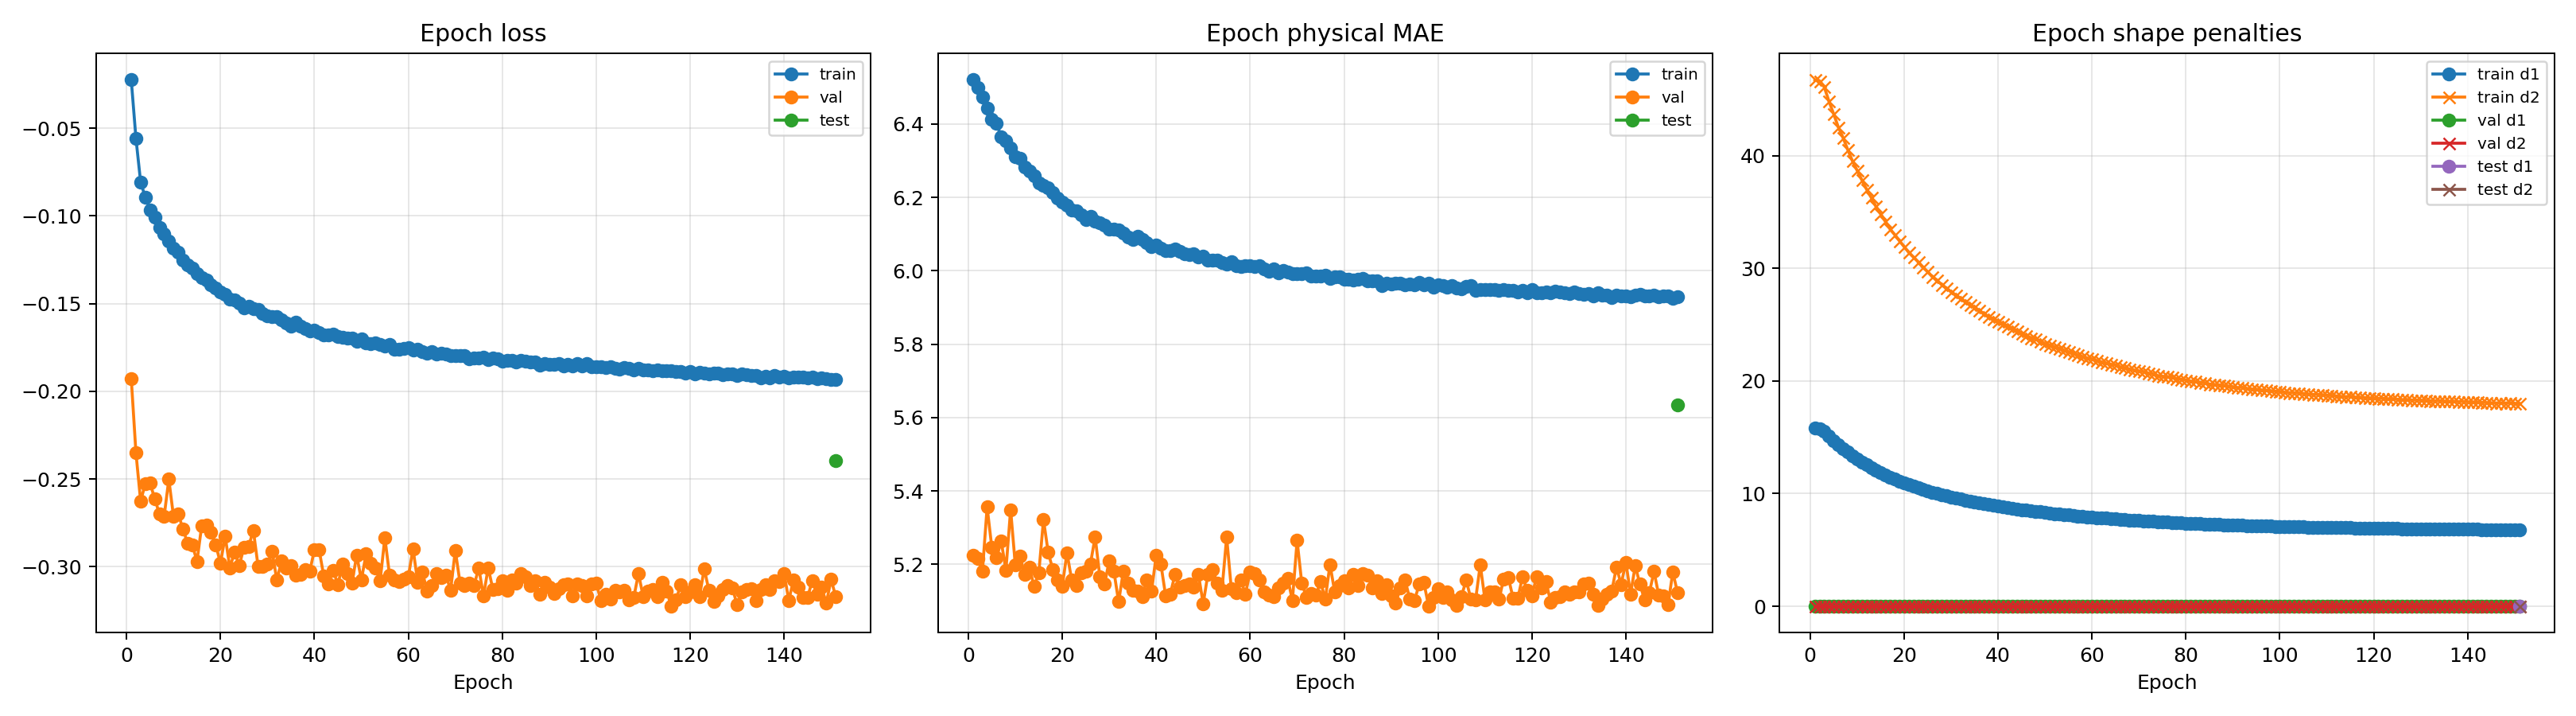
\includegraphics[width=0.85\linewidth]{images/stage2_loss_curves.png}
\caption{Stage-2 NLL training curves showing train and validation Gaussian NLL per epoch. The best validation checkpoint is reached at epoch~116; early stopping halts training at epoch~151.}
\label{fig:stage2-loss-curves}
\end{figure}

\subsubsection{Stage-3 raw-CDF distillation and onset refinement}

The NLL stage produces heteroscedastic predictions that follow the fitted training targets closely, but the fitted curves are not equally faithful over the whole time axis. Near the onset of injection the absolute penetration is small, so any timing offset, fit-delay ambiguity, or smoothness prior produces a relatively large fractional error, and the earliest segment of each predicted curve is shaped primarily by the fitted-target prior rather than by directly observed raw plume dynamics. Figure~\ref{fig:stage2-toy-inference-early-time} shows this in a representative toy-inference sweep.

\begin{figure}[t]
\centering
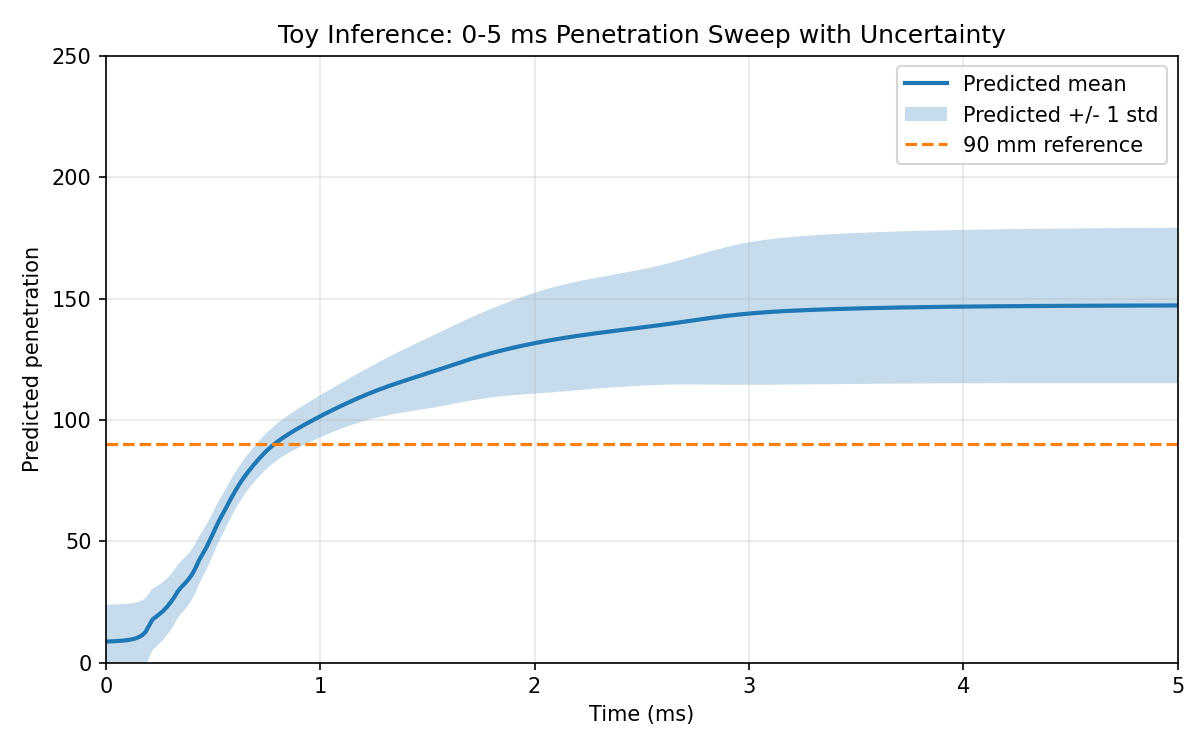
\includegraphics[width=0.82\linewidth]{images/stage2_toy_inference_2000bar_5bar.png}
\caption{Toy inference of the stage-2 NLL model for a representative \(\SI{2000}{bar}\), \(\SI{5}{bar}\) case. The prediction is smooth and well-behaved overall, but the earliest part of the trajectory is still shaped primarily by the fitted-target prior, motivating the subsequent distillation refinement.}
\label{fig:stage2-toy-inference-early-time}
\end{figure}

To refine the early-time dynamics against raw CDF penetration observations while preventing collapse in the late-time sparse regime, a knowledge-distillation stage is introduced on top of the Stage-2 teacher. In population terms, Stage~3 mixes Dataset~\#1 raw observations with the Stage~2 teacher learned from Dataset~\#3. The student network inherits the teacher weights and is further trained on raw CDF penetration together with teacher guidance.

\textbf{CDF penetration coverage regimes.}  Because the raw CDF penetration series are right-censored (by $t\approx\SI{3}{ms}$ many operating conditions have lost more than 70\% of their measurements), direct raw supervision cannot be applied uniformly in time. For each operating-condition group, raw observations are binned in $\Delta t=\SI{0.1}{ms}$ intervals over $[0,5]\,\si{ms}$, and the smoothed sample count per bin determines three mutually exclusive regimes: the high-confidence raw regime (smoothed coverage $\geq70\%$ of peak), the uncertain raw regime (coverage between 20\% and 70\%), and the teacher-only extrapolation regime (coverage below 20\% or fewer than 4 samples per bin). Transitions require at least two consecutive bins in a regime to prevent isolated dips from triggering premature regime changes.

The 70\%/20\% coverage boundaries are conservative engineering regime rules, not optima from a full grid search. The completed Stage~3 ablations support two conclusions: switching off the early anchor reduces global underestimation bias, and retaining mild KD mixing in the reliable raw regime performs better than removing teacher guidance entirely. A systematic sensitivity analysis of the coverage boundaries and \(\sigma_{\mathrm{ref}}\) falls outside the present ablation scope and is acknowledged as a limitation.

\begin{figure}[t]
\centering
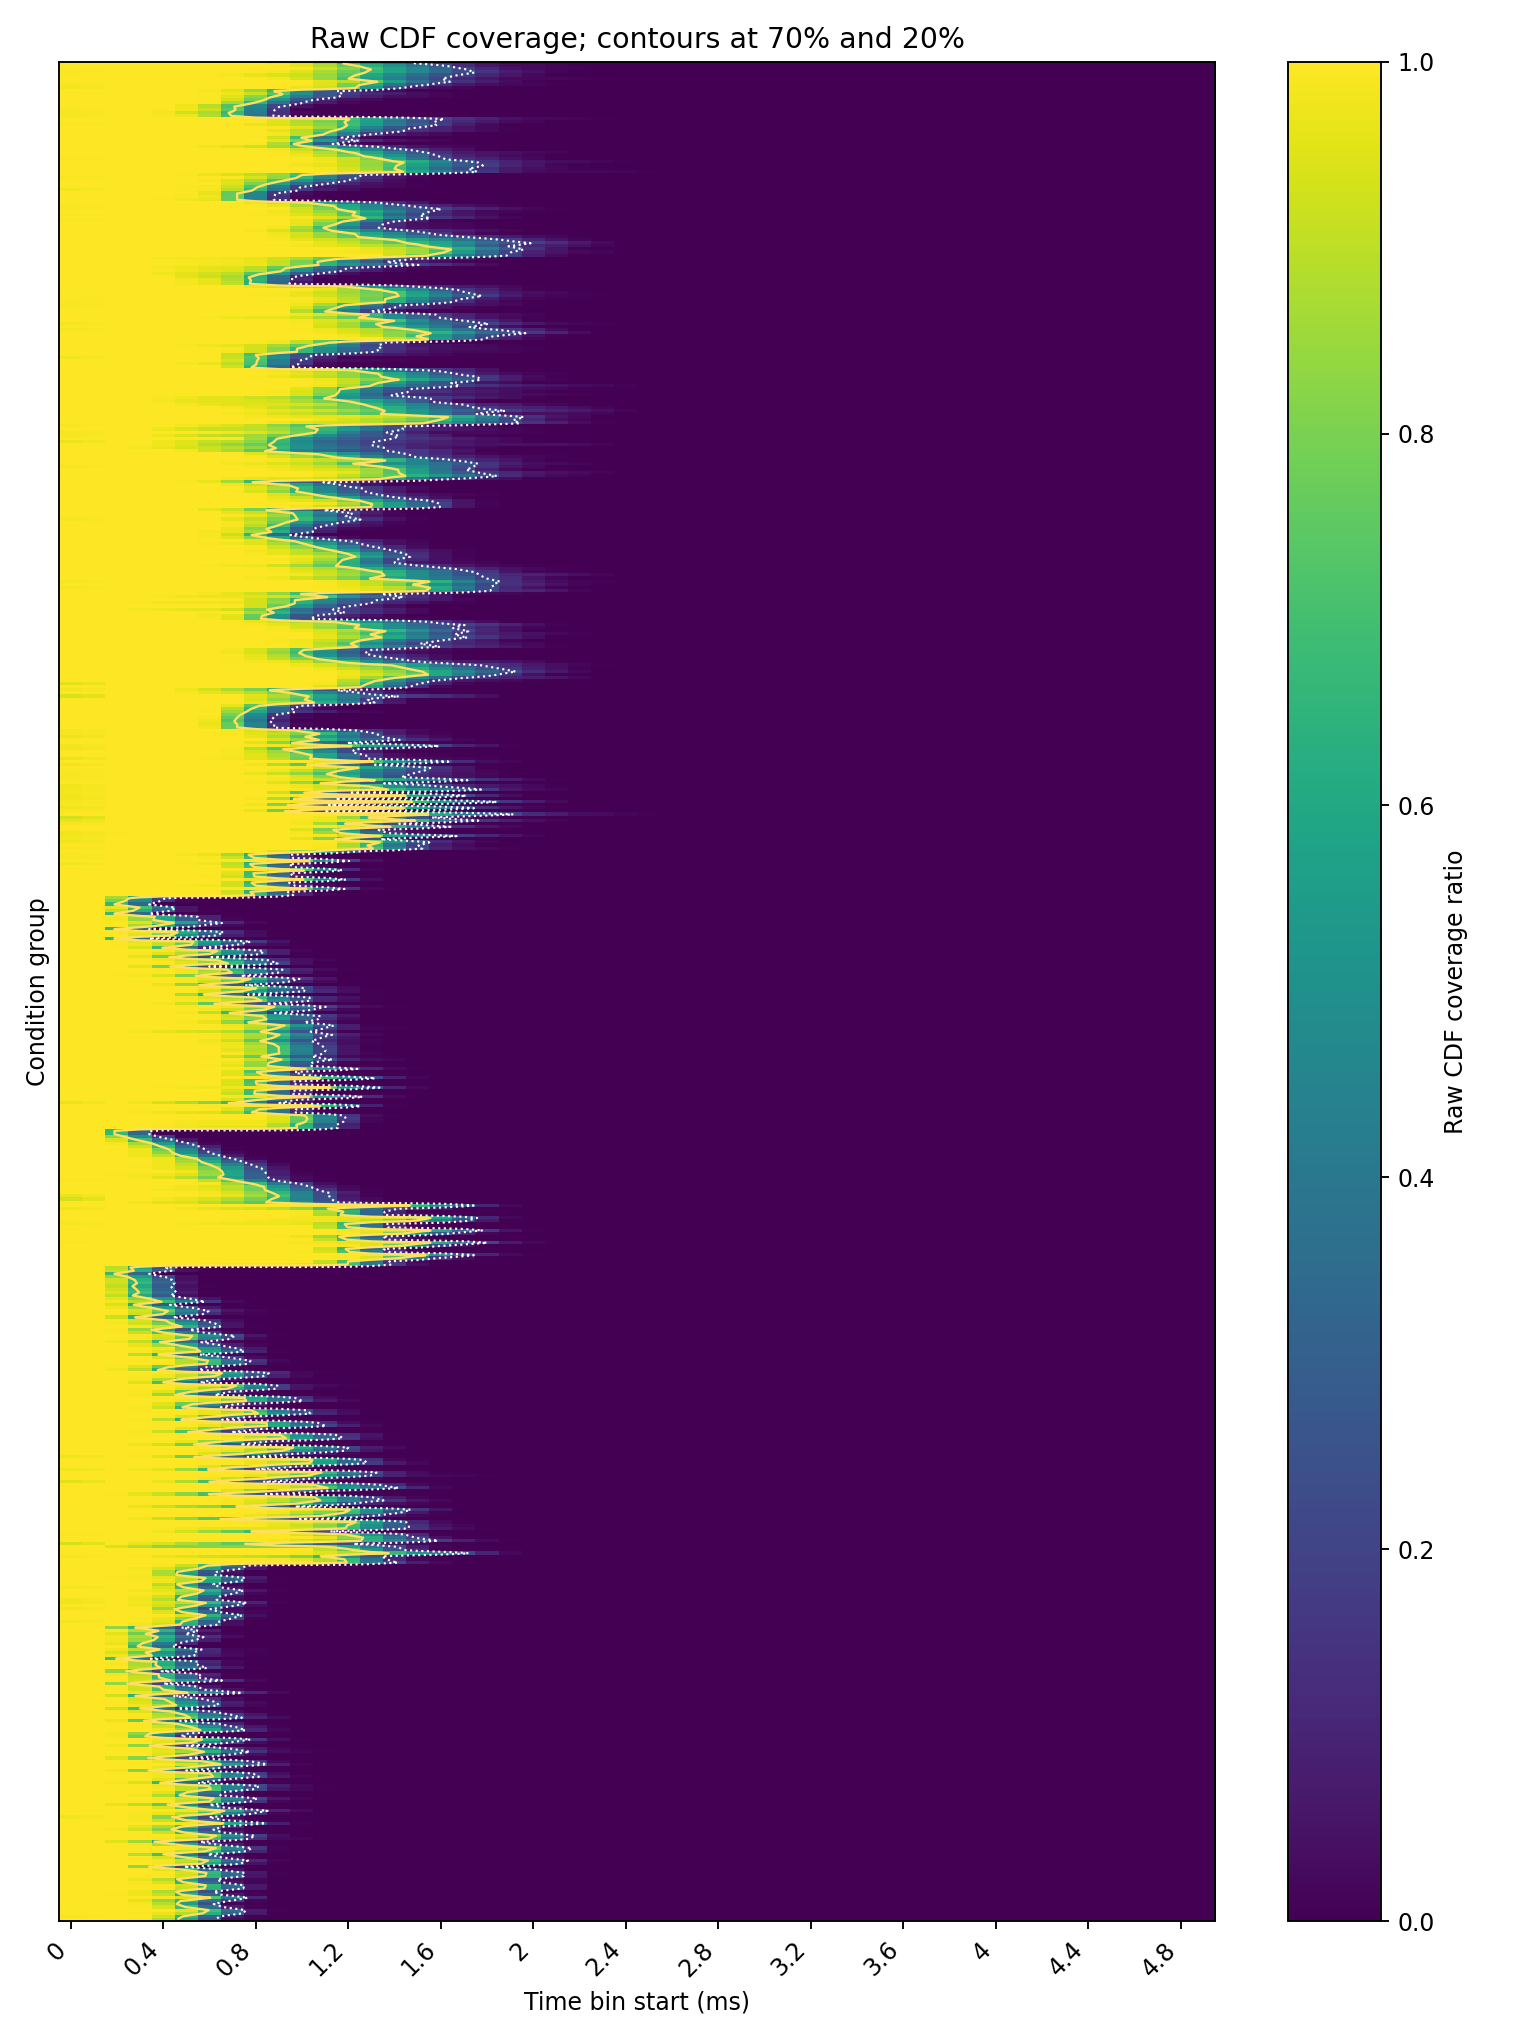
\includegraphics[width=0.94\linewidth]{../generated/current/raw_coverage_heatmap.png}
\caption{Generated raw-CDF coverage heatmap used to audit the 70\%/20\% regime boundaries. Contours mark the reliable-to-uncertain and uncertain-to-teacher-only thresholds.}
\label{fig:raw-coverage-heatmap-generated}
\end{figure}

Figure~\ref{fig:raw-uncertain-teacher-gaussian} shows why this regime split motivates distillation rather than a single-source target. In representative \(\SI{2000}{bar}\), \(\SI{5}{bar}\) cases, the surviving uncertain-regime CDF penetration points still carry useful local information, but they occupy a thinning and biased subset of the teacher's wider predictive distribution. The teacher Gaussian therefore acts as a stabilising continuation of the raw trend rather than as an arbitrary replacement of measured data.

\begin{figure}[p]
\centering
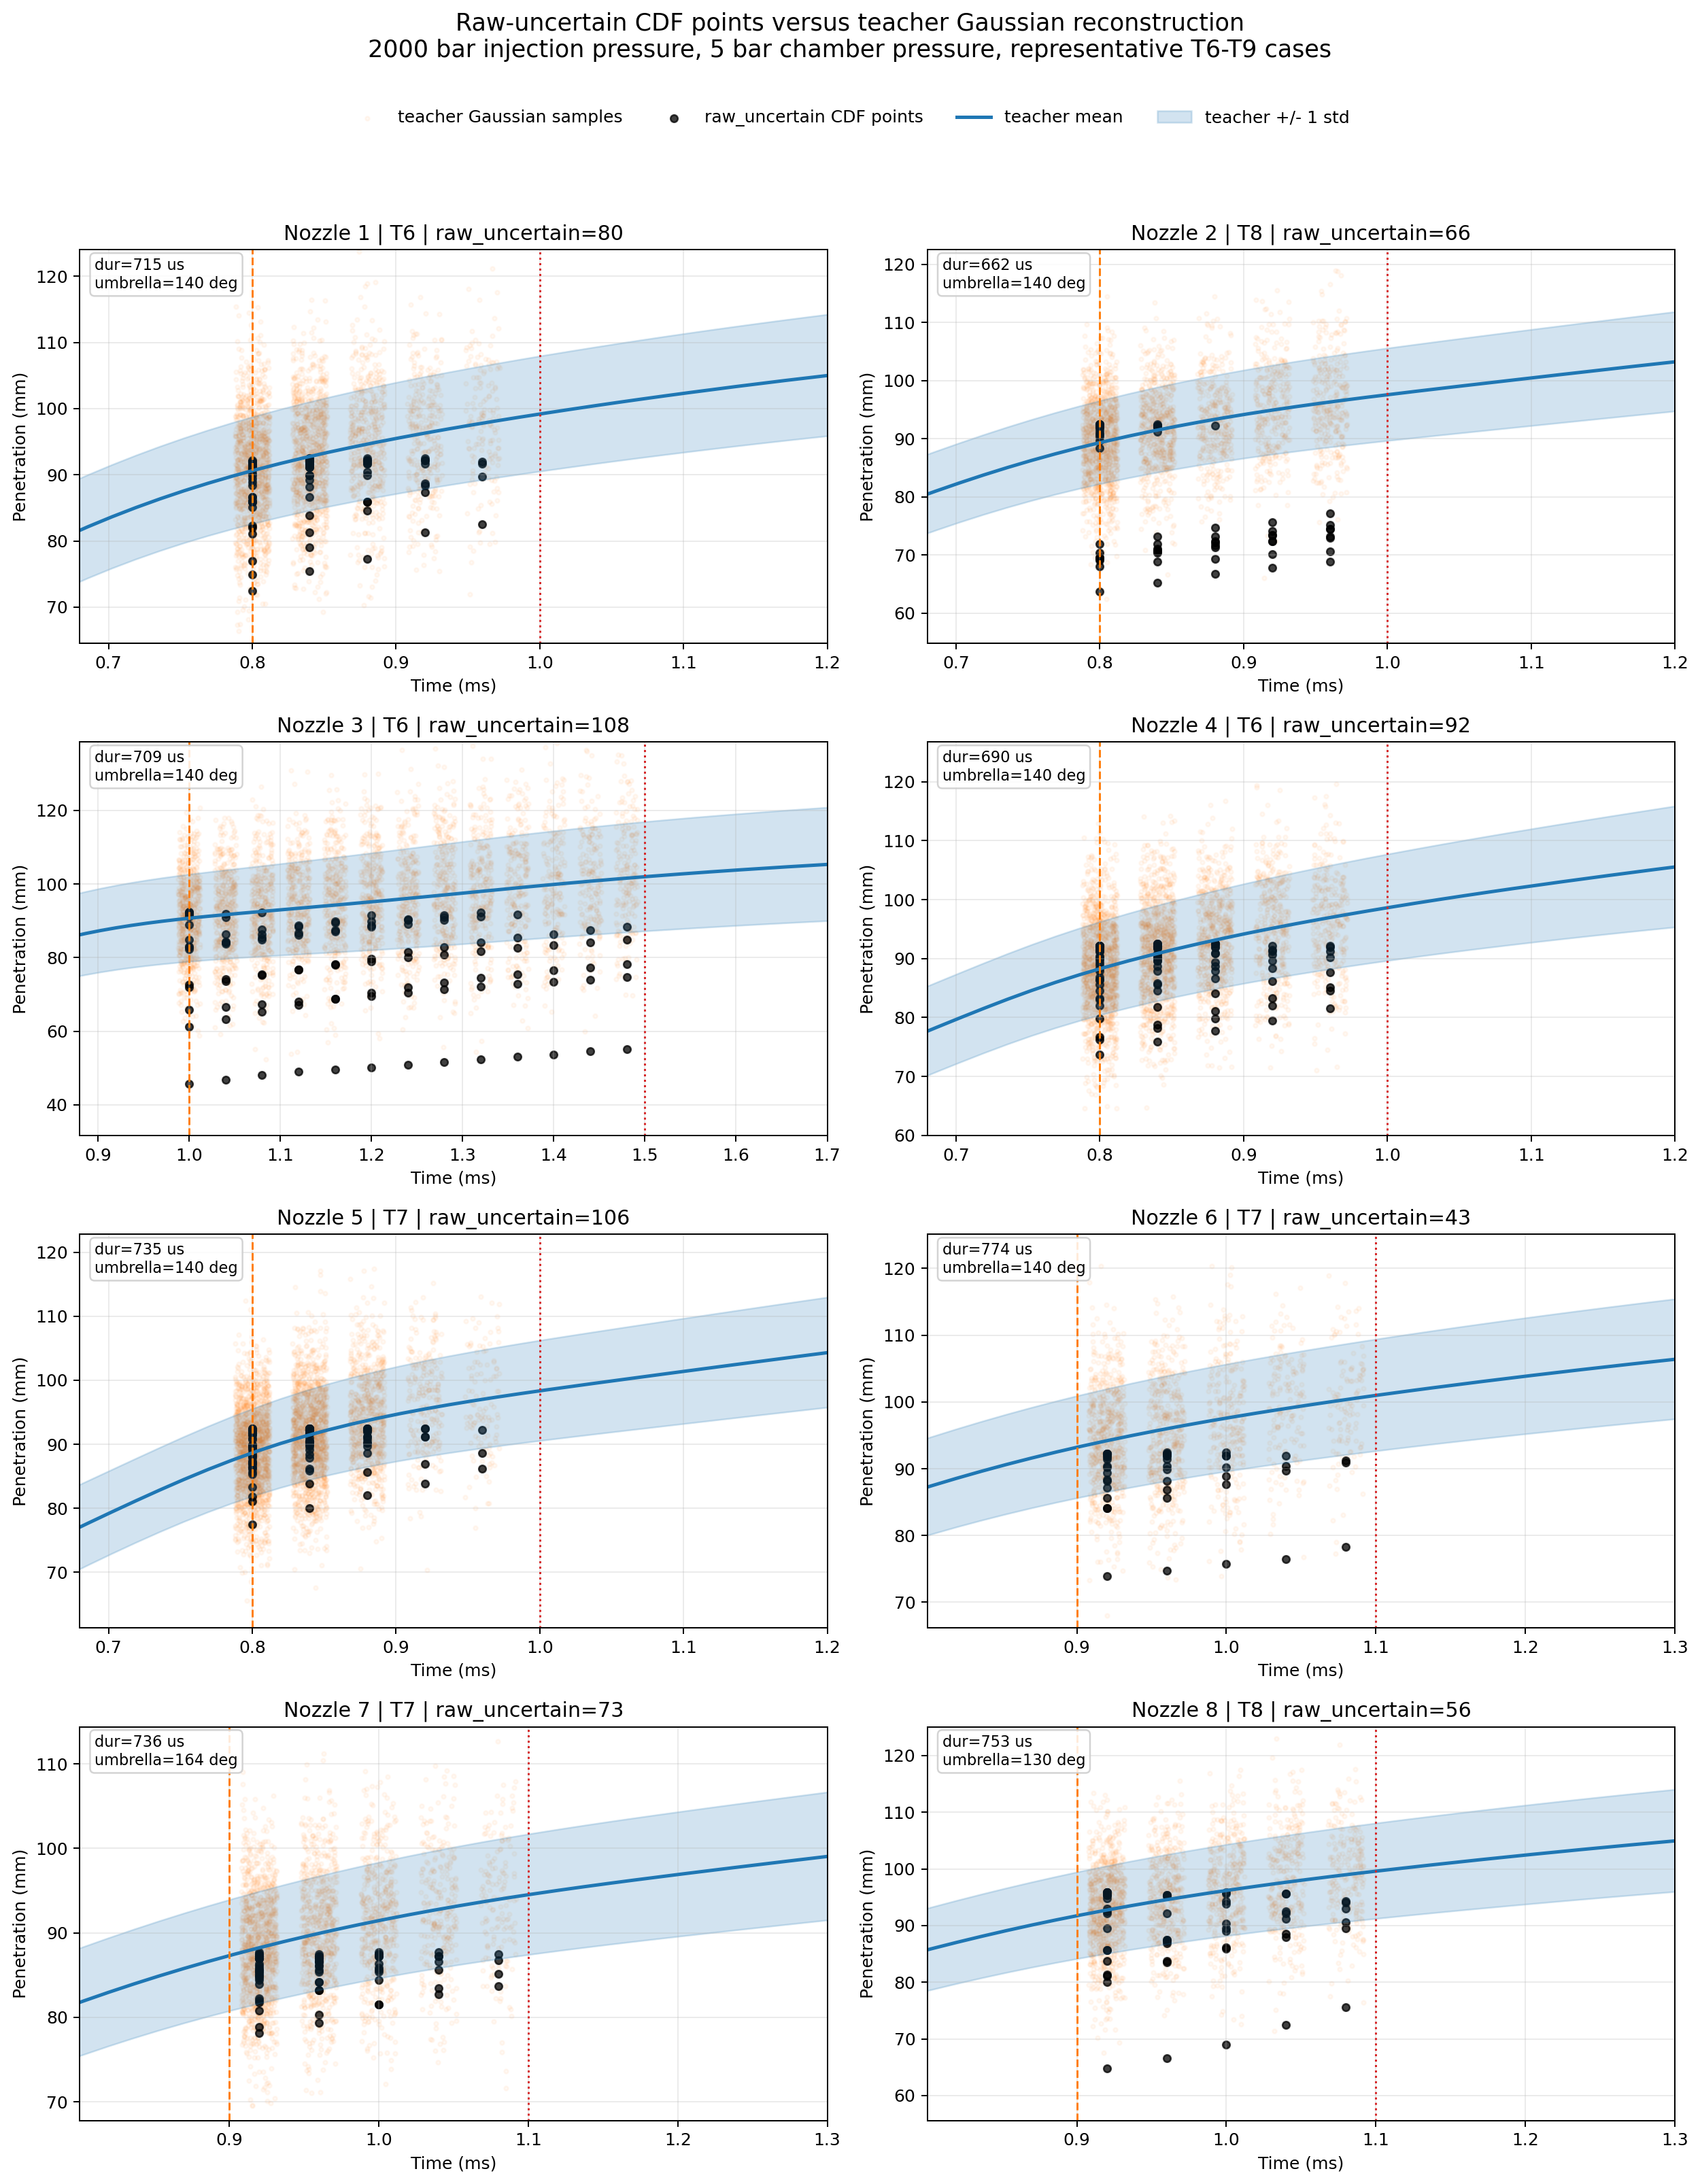
\includegraphics[height=0.88\textheight,keepaspectratio]{images/raw_uncertain_vs_teacher_gaussian_2000bar_5bar.png}
\caption{Representative uncertain-regime CDF penetration points compared with the Stage~2 teacher Gaussian reconstruction for \(\SI{2000}{bar}\) injection pressure and \(\SI{5}{bar}\) chamber pressure. Black points are the surviving raw CDF observations in the uncertain regime, orange points are samples from the teacher Gaussian at the same times, and the blue curve and band show the teacher mean and \(\pm1\sigma\). The plot illustrates why the Stage~3 objective blends raw supervision with teacher guidance once coverage begins to collapse.}
\label{fig:raw-uncertain-teacher-gaussian}
\end{figure}

\textbf{Supervision weights.}  Each grid point receives two independent weight channels:

\begin{center}
\begin{tabular}{lcc}
\toprule
Regime & Raw weight $w_{\mathrm{raw}}$ & KD weight $w_{\mathrm{kd}}$ \\
\midrule
the high-confidence raw regime  & 1.0 & 0.25 \\
the uncertain raw regime & 0.0 & 1.0  \\
the teacher-only extrapolation regime  & 0.0 & 0.75 \\
\bottomrule
\end{tabular}
\end{center}

Both channels are further modulated by a global time-bin rebalancing weight (inverse-frequency, clipped to $[0.5,2.0]$). In the high-confidence raw regime bins, raw NLL is the primary signal with mild KD regularisation. In the uncertain raw regime bins, raw supervision is dropped and teacher KD MSE dominates. In the teacher-only extrapolation regime bins, the KD weight is slightly reduced to acknowledge teacher extrapolation uncertainty. Two single-run checks support this regime filter: replacing \texttt{series\_wide\_clean} with a pre-truncated raw source changes RMSE negligibly (\(\Delta\mathrm{RMSE}\approx-\SI{0.003}{mm}\)), while disabling the low-confidence raw-weight filter degrades RMSE by about \(\SI{0.065}{mm}\). The latter is small but directionally important: treating right-censored late frames as ordinary raw supervision is measurably worse than deferring to the teacher in those bins.

\textbf{Composite loss.}  The training objective is
\[
\mathcal{L} = \mathcal{L}_{\mathrm{raw}} + \mathcal{L}_{\mathrm{KD}} + \lambda_{\mathrm{onset}}\,\mathcal{L}_{\mathrm{onset}} + \lambda_{\mathrm{anchor}}\,\mathcal{L}_{\mathrm{anchor}} + \lambda_{d_1}\,P_{d_1} + \lambda_{d_2}\,P_{d_2},
\]
where $\mathcal{L}_{\mathrm{raw}}$ is the Gaussian NLL on physical $(\mu,\sigma^2)$ against raw CDF penetration targets weighted by $w_{\mathrm{raw}}$; $\mathcal{L}_{\mathrm{KD}}$ is a hybrid MSE on means and log-variances in physical space, weighted by $w_{\mathrm{kd}}$:
\[
\mathcal{L}_{\mathrm{KD}} = \mathrm{MSE}(\mu_s,\,\mu_t) + \lambda_\sigma\,\mathrm{MSE}(\log\sigma^2_s,\,\log\sigma^2_t),\qquad \lambda_\sigma = 5.0;
\]
$\mathcal{L}_{\mathrm{onset}}$ is a binary cross-entropy loss on a new onset logit output against a ramp target $\min(t/t_{\mathrm{ramp}},1)$ active only for $t\leq\SI{0.2}{ms}$ ($\lambda_{\mathrm{onset}}=0.1$); $\mathcal{L}_{\mathrm{anchor}}$ is a quadratic penalty pulling $\mu(t\approx0)$ toward zero, ramping down over the first \SI{0.15}{ms}. This anchor term is retained in the general objective and in the baseline run ($\lambda_{\mathrm{anchor}}=0.01$), but the final selected checkpoint sets $\lambda_{\mathrm{anchor}}=0$ after the ablation evidence below showed that the anchor introduced a small systematic under-prediction. $P_{d_1}=\operatorname{ReLU}(-\Delta\mu)^2$ enforces monotonicity; and $P_{d_2}=\operatorname{ReLU}(+\Delta^2\mu)^2$ enforces concavity for $t\geq\SI{0.5}{ms}$.

\begin{table}[t]
\centering
\footnotesize
\setlength{\tabcolsep}{3pt}
\renewcommand{\arraystretch}{1.18}
\begin{tabular}{@{}L{0.12\linewidth}L{0.24\linewidth}L{0.24\linewidth}L{0.30\linewidth}@{}}
\toprule
Stage & Data-fit and variance/onset terms & Shape priors & Gating and distillation parameters \\
\midrule
Stage~1 &
\(\lambda_{\mathrm{var}}=10^{-3}\), \(c_0=-2\) &
\(\lambda_1=5\times10^{-5}\), \(\lambda_2=5\times10^{-4}\) &
\(t_c=\SI{0.9}{ms}\), \(\tau_c=\SI{0.05}{ms}\) \\
Stage~2 &
heteroscedastic NLL, \(\log\hat{\sigma}^2\in[-10,6]\); early-time anchor \(\lambda_\mu=10^{-2}\), \(\lambda_\sigma=0\) (window \(\tau=\SI{0.15}{ms}\), selected from Section~\ref{sec:stage2-anchor-ablation-en}) &
\(\lambda_1=5\times10^{-5}\), \(\lambda_2=5\times10^{-5}\) &
\(t_c=\SI{0.5}{ms}\), \(\tau_c=\SI{0.05}{ms}\) \\
Stage~3 &
\(\lambda_{\mathrm{onset}}=0.1\), final \(\lambda_{\mathrm{anchor}}=0\) &
\(\lambda_{d_1}=5\times10^{-5}\), \(\lambda_{d_2}=5\times10^{-4}\) &
\(t_c=\SI{0.5}{ms}\), \(\tau_c=\SI{0.05}{ms}\), \(\lambda_\sigma=5.0\); \(w_{\mathrm{raw}}=(1.0,0,0)\), \(w_{\mathrm{kd}}=(0.25,1.0,0.75)\) \\
\bottomrule
\end{tabular}
\caption{Reproducibility-relevant hyperparameters for the three training stages. Stage~1/2 values are taken from the corresponding training-config snapshots; Stage~3 values are from the final anchor-off run. The \(w_{\mathrm{raw}}\) and \(w_{\mathrm{kd}}\) triples are ordered as (high-confidence raw regime, uncertain raw regime, teacher-only extrapolation regime).}
\label{tab:training-hyperparameters}
\end{table}

\textbf{Student architecture.}  The student is a three-output MLP extending the teacher's two outputs $[\hat\mu,\;\log\hat\sigma^2]$ with an onset logit. All shared layers are copied from the teacher checkpoint; the final linear row for the onset head is initialised to zero (sigmoid $\to0.5$). All losses are computed in physical space by multiplying student and teacher outputs by the per-sample $A$ before evaluating $\mathcal{L}_{\mathrm{KD}}$, $\mathcal{L}_{\mathrm{raw}}$, and the shape priors.

\textbf{Training and results.}  The student is optimised with the decoupled-weight-decay adaptive-moment optimiser at $\mathrm{lr}=3\times10^{-3}$ with gradient clipping at norm~1.0 and early stopping with patience~20. In the selected anchor-off configuration, the best validation composite loss is~2.389 (val raw NLL~1.972, val KD MSE~0.374, val onset BCE~0.427). On the held-out test set, the composite loss is~2.396, with raw NLL~1.988, KD MSE~0.366, onset BCE~0.427, and negligible derivative penalties ($P_{d_1}\approx3.0\times10^{-12}$, $P_{d_2}\approx1.8\times10^{-6}$). Figure~\ref{fig:distillation-loss} shows the training curves; the downstream screening performance of this checkpoint is reported in Table~\ref{tab:model-summary}.

These Stage~3 loss values are not directly comparable to the Stage~2 scaled NLL. Stage~2 optimises fitted q1 targets on the filtered trajectory table, whereas Stage~3 mixes raw CDF penetration likelihood, teacher--student KD MSE, onset supervision, and shape penalties on a different raw/KD-regime population. The reproducibility pipeline therefore exports each stage metric with an explicit target-population label rather than placing all NLL-like numbers on a single leaderboard.

\begin{figure}[t]
\centering
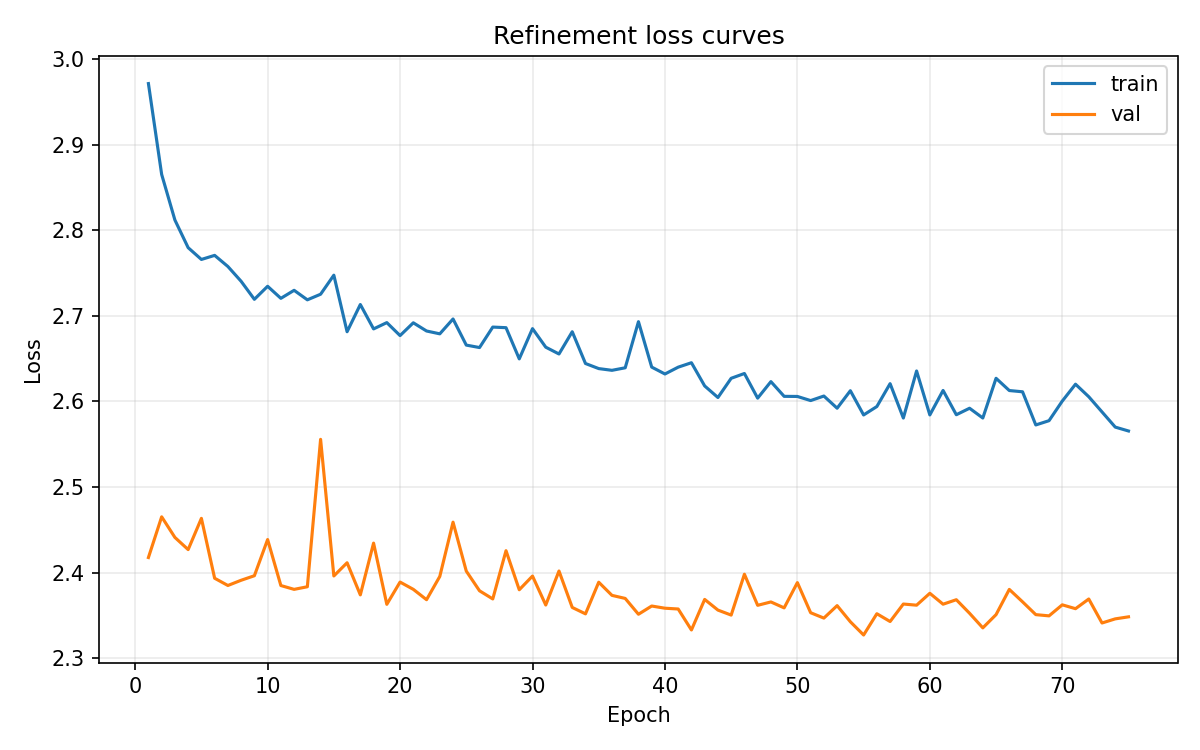
\includegraphics[width=0.92\linewidth]{images/distillation_loss_curves.png}
\caption{Distillation stage training curves for the selected anchor-off Stage~3 run. The composite loss reaches its best validation value of~2.389.}
\label{fig:distillation-loss}
\end{figure}

The three-stage surrogate constructed above is compared against physical baselines and a kernel-based alternative backbone in Chapter~5. The following subsections separate those roles: the sparse GP is treated as an alternative probabilistic regressor for the same low-dimensional scaled task, while Hiroyasu--Arai and Naber--Siebers remain empirical physical baselines.

\subsection{Sparse heteroscedastic GP as an alternative surrogate backbone}
\label{sec:svgp-alternative-backbone-en}

The sparse heteroscedastic Gaussian-process model should be read as a strong alternative surrogate backbone rather than as a weak baseline. It solves the same low-dimensional regression problem as the MLP: the target is the non-dimensional penetration \(\hat S=S/A\), predictions are converted back to millimetres through \(A\hat\mu\) and \(A\hat\sigma\), and the evaluation uses the same CDF observable and fixed tables. The GP differs in its inductive bias, not in the physical target.

The implemented GP uses the ``a-only'' five-feature set,
\[
[\,t_{\mathrm{norm}},\;\theta_{\mathrm{tilt},z},\;n_{\mathrm{plumes},z},\;t_{i,z},\;P_{\mathrm{cb},z}\,],
\]
with the dominant pressure, density, and diameter dependence absorbed into \(A\). It is sparse and heteroscedastic: one sparse variational GP learns the conditional mean, and a second sparse variational GP learns the log residual variance. Both use a Mat\'ern \(5/2\) kernel with automatic-relevance-determination length scales, while inducing-point variational inference makes the problem feasible on the million-point Stage~3 training table.

This architecture is especially natural for the present task because the input space is low-dimensional and the desired function is smooth. In both the refreshed in-distribution comparison and the leave-one-nozzle-family stress test reported in Chapter~5, the SVGP is the stronger point predictor. Its kernel prior also gives a more graceful failure mode when a held-out nozzle family lies outside the support of the training matrix: away from data, the posterior is constrained by the kernel and inducing-point structure rather than freely extending a learned nonlinear surface.

The MLP is still retained as the main protocol instantiation for three reasons. First, the Stage~3 student carries an onset side head used by the screening interface; the current SVGP replaces the penetration \((\mu,\sigma)\) regressor but not that side channel. Second, the MLP implements the regime-aware raw/KD training chain directly, making it easy to combine Dataset~\#1 raw observations and the Dataset~\#3 teacher in one lightweight network. Third, the MLP makes the feature, anchor, and distillation ablation matrices affordable on a high-performance workstation PC. The engineering conclusion is therefore conditional: choose SVGP when point RMSE/MAE in interpolation or nozzle-family transfer is the priority; choose the MLP stack when conservative screening, onset output, deployment simplicity, and design-attribution ablations are the priority.

\subsection{Physical baselines and evaluation protocol}
\label{sec:baseline-fitting-protocol-en}

The Hiroyasu--Arai and Naber--Siebers baselines reported in the results chapter are built from the same external-cleaning evaluation table, rather than being fitted directly to raw image pixels.
The comparison therefore tests different penetration function families under the same observable definition and data split; it does not mix different image-processing methods.
On the image side, the input first passes through the common workflow described in Chapter~3: nozzle-centre calibration, polar plume-strip extraction, background and gradient enhancement, per-plume axial intensity projection, CDF-front quantile extraction, abnormal-jump truncation, short-segment removal, pixel-to-millimetre conversion, and SOI / hydraulic-delay time alignment.
The baseline models then receive pointwise penetration \(S(t)\), the corresponding standardised operating-condition features, and canonical physical quantities such as \(d_n\), \(\Delta P\), \(\rho_a\), and \(A\) derived from the test-matrix JSON files.

The Hiroyasu--Arai baseline uses the two-stage function \(S_{\mathrm{HA}}(t)\) described in the literature review.
The ``calibrated'' row in the results table does not simply reuse literature constants; it fits the log-parameters of \((k_v,k_p,k_b)\) on the training split with Huber robust least squares, then evaluates fixed parameters on validation and test splits.
The log-parameterisation keeps the gains and breakup-time scale positive, while the Huber loss reduces the leverage of a small number of image-derived outliers on the global empirical law.
The Naber--Siebers baseline uses the delayed square-root form \(S_{\mathrm{NS}}(t)=k_{\mathrm{NS}}A\sqrt{\max(t-\tau,0)}\), with \(A=(\Delta P/\rho_a)^{1/4}d_n^{1/2}\).
The reported row fits \(\log k_{\mathrm{NS}}\) and \(\tau\), with the delay bounded to \([-0.1,0.8]\,\si{ms}\); the angle correction exists only as an optional implementation path, and the final comparison uses neither training-set cone angles nor oracle cone angles.

To make the physical baselines usable in probabilistic evaluation, their uncertainty is not assigned as an arbitrary constant.
After fitting, training/validation residuals are binned in time at \(\SI{0.1}{ms}\), and the robust spread is estimated with \(1.4826\,\mathrm{MAD}\), with a floor of \(\SI{0.5}{mm}\) to avoid unrealistically narrow bands in sparse early bins.
This \(\sigma(t)\) lets the empirical laws report 1\(\sigma\), 2\(\sigma\) coverage and CRPS while retaining their traditional penetration-correlation mean functions. The sparse GP described in Section~\ref{sec:svgp-alternative-backbone-en} is evaluated on the same tables, but it is interpreted as an alternative probabilistic surrogate backbone rather than as a traditional physical baseline.

\begin{table}[t]
\centering
\footnotesize
\setlength{\tabcolsep}{3pt}
\begin{tabular}{@{}L{0.18\linewidth}L{0.25\linewidth}L{0.25\linewidth}L{0.24\linewidth}@{}}
\toprule
Physical baseline & Target and inputs & Fitted quantities & Probabilistic output \\
\midrule
Calibrated Hiroyasu--Arai &
Image-CDF penetration \(S(t)\); \(t,d_n,\Delta P,\rho_a\) &
\(\log k_v,\log k_p,\log k_b\), Huber robust least squares &
Time-binned residual MAD; \(\sigma_{\min}=\SI{0.5}{mm}\) \\
\midrule
Delayed Naber--Siebers &
\(S(t)\); \(t,A=(\Delta P/\rho_a)^{1/4}d_n^{1/2}\) &
\(\log k_{\mathrm{NS}}\) and \(\tau\in[-0.1,0.8]\,\si{ms}\) &
Same residual-binning protocol; no oracle cone angle \\
\bottomrule
\end{tabular}
\caption{Unified construction protocol for the traditional physical baselines in the external-cleaning evaluation. Both empirical laws use the same image-derived CDF penetration table, group-aware split, and evaluation target as the MLP and SVGP surrogates.}
\label{tab:baseline-fitting-protocol-en}
\end{table}

\subsubsection{Evaluation protocol and metrics}
\label{sec:evaluation-protocol-en}

All models are evaluated on common held-out tables derived from the external-cleaning evaluation procedure described above. The procedure re-runs the full image-processing and target-construction chain on a frozen image archive and produces penetration tables that are then partitioned group-wise into training, validation, and test splits. The test partition is never used for model selection or hyperparameter tuning; reported test-set numbers are therefore single evaluations on data the model has not influenced.

Four evaluation views are kept separate because they answer different questions. The full-clean CDF protocol measures overall point accuracy on the common cleaned CDF set, including right-censored regions. The conservative uncensored CDF protocol removes bins beyond the density-drop or FOV-saturation thresholds from Dataset~\#2 and is the main physical point-level metric for censoring-controlled comparison. The P50 observed protocol compresses each condition to median observed penetration points, testing the robustness of the mean head against plume-to-plume scatter. The Q1 extrapolated protocol evaluates model predictions on the companion q1 grid fitted to the P50 trace; it is an extrapolation diagnostic, not an independent ground truth.

\textbf{Point-error metrics.} Root-mean-square error (RMSE) and mean absolute error (MAE) measure the accuracy of the predicted conditional mean $\mu(t)$ against held-out pointwise penetration observations. Both are computed over the full time range covered by the test trajectories. Because errors within a single trajectory are temporally correlated, the effective sample size is substantially smaller than the raw point count, and reported values characterise average per-point error across a heterogeneous population of operating conditions and time instants rather than a statistically independent sample.

\textbf{Empirical coverage.} A heteroscedastic model outputs both a conditional mean $\mu(t)$ and a conditional standard deviation $\sigma(t)$. The primary calibration question is whether the predicted uncertainty intervals are empirically trustworthy: under a Gaussian predictive distribution, $68.3\%$ of observations should fall within the $[\mu-\sigma,\,\mu+\sigma]$ interval and $95.4\%$ within the $[\mu-2\sigma,\,\mu+2\sigma]$ interval. The empirical $1\sigma$ coverage on the held-out test set is the primary calibration metric for each probabilistic model: values above $68.3\%$ indicate conservative (over-dispersed) intervals, values below indicate over-confident (under-dispersed) predictions. For the physical baselines, $\sigma(t)$ is the time-binned robust residual spread estimated from training residuals; for the MLP stages, $\sigma(t)$ is the network's direct output.

\textbf{Continuous ranked probability score.} The CRPS evaluates the predictive cumulative distribution function $F$ against a scalar observation $y$ as
\[
\mathrm{CRPS}(F,y) = \int_{-\infty}^{\infty}\!\left(F(z)-\mathbf{1}[z\geq y]\right)^2\mathrm{d}z.
\]
Under a Gaussian predictive distribution with mean $\mu$ and standard deviation $\sigma$ this reduces to a closed-form expression that simultaneously rewards accuracy (small $|\mu-y|$) and calibration (neither too wide nor too narrow $\sigma$). Lower CRPS is better; a perfectly sharp and accurate point forecast has $\mathrm{CRPS}=0$.

\textbf{Reliability, ECE, and PIT.} For every prediction, the observation can be converted into a predictive percentile,
\[
u_i=\Phi\!\left(\frac{y_i-\mu_i}{\sigma_i}\right).
\]
If the Gaussian predictive distributions are calibrated, the \(u_i\) values should be uniformly distributed on \([0,1]\). Reliability diagrams compare nominal lower-tail probability with the empirical fraction of points below that percentile, while expected calibration error averages the absolute deviation across a grid of probability levels. PIT histograms show the same information visually: U-shaped histograms indicate under-dispersion, hump-shaped histograms indicate over-dispersion, and skew indicates mean bias. Because the full-clean table contains hundreds of thousands of temporally correlated points, KS \(p\)-values are treated as sensitivity indicators rather than as binary pass/fail labels; the histogram shape, ECE, and coverage curves carry the engineering interpretation.

\textbf{Leave-one-nozzle-family evaluation.} The standard group-aware split retains all nozzle families in the training and validation partitions and evaluates interpolation across pressure and duration combinations within the supported operating domain. To probe out-of-distribution robustness in a physically meaningful direction, a secondary leave-one-nozzle-family evaluation is also conducted: all operating conditions belonging to one nozzle family are removed from the training and validation splits, the model is retrained on the remaining families, and performance is evaluated on the held-out family alone. This procedure is repeated for each nozzle family in turn. Because nozzle families differ in hole diameter, plume count, and early-transient spray formation dynamics, the leave-one-family test asks whether the staged architecture generalises to a nozzle geometry never seen during training — the most demanding interpolation scenario the present dataset can provide. Results from both evaluation protocols are reported in Chapter~5.

\subsection{Probabilistic screening interface}
\label{sec:screening-interface-en}

The literature-review discussion of spray--wall impingement mechanisms concluded that the appropriate downstream object for an uncertainty-aware penetration surrogate is a probabilistic screening proxy rather than a binary pass/fail rule, and that penetration should be projected onto the engine-geometry plane as a rotated two-dimensional Gaussian before being integrated against cylinder-wall and piston-crown masks. The current GUI prototype operationalises that proxy by coupling the final Stage-3 student checkpoint to a parametric piston crown, cylinder wall, and slider-crank displacement model, then exporting spatial snapshots, probability time histories, cumulative exposure, and an animation. The MLP is currently the most complete drop-in model for this interface because it provides both penetration \((\mu,\sigma)\) and the onset side head used in the diagnostic plots. The SVGP from Section~\ref{sec:svgp-alternative-backbone-en} can replace the penetration mean and variance in the same geometric integral, but it does not directly replace the onset head without an additional side model. The default configuration uses the Design~A piston, \(\mathrm{RPM}=250\), crank phase \(0^{\circ}\), a 0--\SI{5}{ms} time window, and a 60-frame time grid.

\textbf{Spray probability density.}  Let the per-plume spray axis be rotated by $\theta_{\mathrm{tilt}}$ from the radial direction and let $\alpha$ denote the half-cone angle. In the plume-aligned frame, the student prediction supplies an axis-parallel standard deviation $\sigma_{\parallel}(t)$, while the lateral spread is represented by a second Gaussian. The current implementation does not set the lateral standard deviation equal to the geometric half-width directly; it interprets the fixed half-cone angle as an approximate three-standard-deviation envelope and adds a grid-size floor:
\[
\sigma_{\perp}(t)
=\max\!\left\{
\frac{\max\!\left(\mu_{+}(t),\sigma_{\parallel}(t)\right)\tan(\alpha/2)}{3},
\;2\Delta x
\right\},\qquad
\mu_{+}(t)=\max(\mu(t),0).
\]
Here \(\Delta x\) is the grid spacing, defaulting to \(\SI{0.25}{mm/px}\). The floor prevents the lateral PDF from collapsing non-physically near injection onset when \(\mu(t)\) is small, while the factor of \(1/3\) treats the geometric cone angle as an approximate \(3\sigma\) envelope — an engineering convention for probabilistic collision screening rather than a value calibrated against measured spray widths. This fixed-\(\alpha\) assumption is suitable only for early screening and ranking, not as a validated time-varying spray-envelope model. The joint density
\[
p(x,y,t)=\mathcal{N}\!\Bigl((x,y);\,\mathbf{c}(t),\,\mathbf{R}(\theta_{\mathrm{tilt}})\,\operatorname{diag}\!\bigl(\sigma_{\parallel}^{2}(t),\sigma_{\perp}^{2}(t)\bigr)\,\mathbf{R}(\theta_{\mathrm{tilt}})^{\top}\Bigr),
\]
with centre $\mathbf{c}(t)=\mathbf{x}_{\mathrm{nozzle}}+\mathbf{R}(\theta_{\mathrm{tilt}})\,(\mu_{+}(t),0)^{\top}$, is evaluated on a regular canvas grid (default \SI{0.25}{mm/px} over a $125\times\SI{200}{mm}$ window, with the cylinder wall at \(x=\SI{120}{mm}\)) and renormalised per frame so that $\iint p\,\mathrm{d}A=1$. The student's scaled outputs are denormalised to physical space via the empirically calibrated amplitude $A=\Delta P^{0.5}\cdot\rho_a^{-0.25}\cdot d_n^{0.5}$ introduced for the engineered-feature architecture above, so that $\mu$ and $\sigma_{\parallel}$ enter the PDF in millimetres.

\begin{figure}[t]
\centering
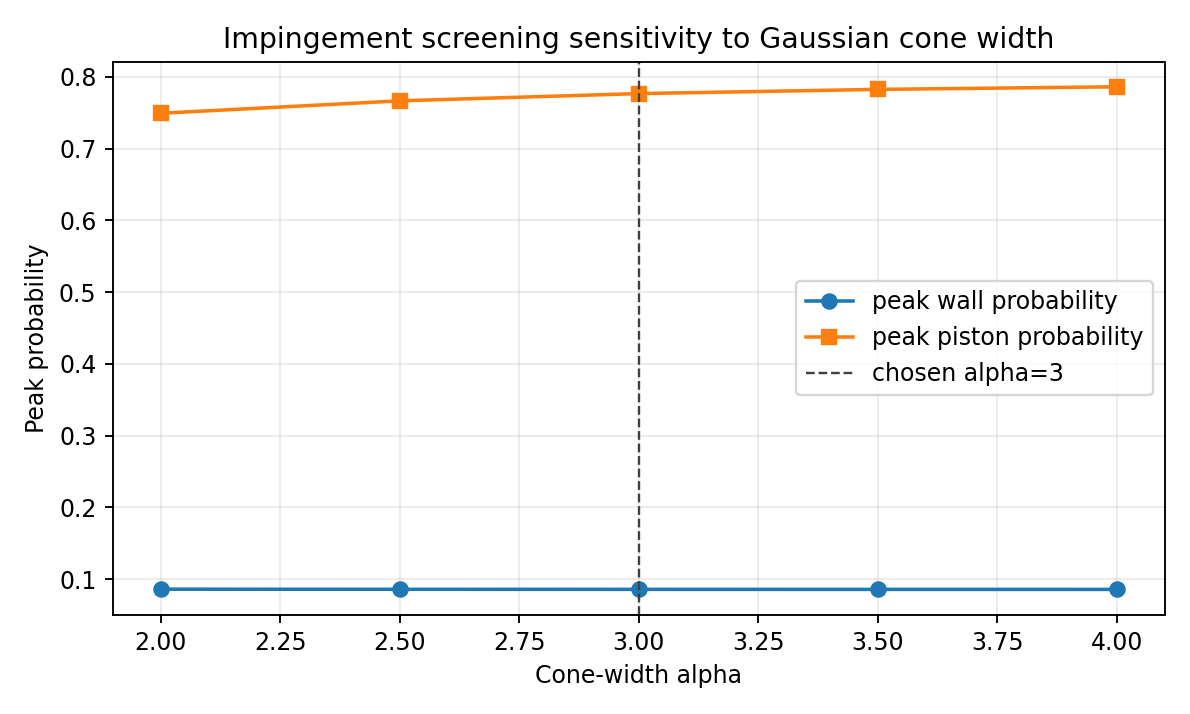
\includegraphics[width=0.82\linewidth]{../generated/current/alpha_sensitivity_figure.png}
\caption{Generated sensitivity sweep for the lateral Gaussian cone-width factor. The selected \(3\sigma\) interpretation is marked against neighbouring \(\alpha\) values to show how strongly the screening probabilities depend on this modelling convention.}
\label{fig:alpha-sensitivity-generated}
\end{figure}

\textbf{Piston geometry dispatcher.}  The prototype exposes three interchangeable crown profiles. The default Design~A is a piecewise-arc construction that assembles a bowl-shaped crown from five circular-arc radii --- outer bowl, inner bowl, topland, lip, and floor --- with hard closure constraints that keep the geometry consistent when any radius is changed. Design~B is a two-arc bowl profile with tangent constraints. The Hermite variant replaces the arc construction with a \emph{quintic Hermite spline} defined by a small set of control points, each carrying a position, a tangent vector, and a second-derivative vector in the (radial, depth) cross-section plane. Matching position, slope, and curvature at every knot gives $C^{2}$ continuity across segment boundaries, so the crown surface has no curvature jumps --- a property relevant both for CNC machining (where curvature discontinuities translate into tool-acceleration steps) and for the collision-integral mesh (where abrupt curvature changes could alias onto the rasterised mask).

The parameterisation also makes systematic parameter sweeps straightforward: varying a single scalar --- the nadir depth, for example --- continuously deforms the entire bowl profile while the rest of the control-point structure adapts through the spline, without requiring any constraint equations to be re-solved. Figure~\ref{fig:hermite-crown} illustrates the baseline four-point crown together with its tangent arrows (panel~a) and a seven-level nadir-depth sweep (panel~b) that demonstrates the continuous, smooth deformation produced by changing one parameter. All three designs return a binary piston mask on the same canvas grid as the spray density; the latest default GUI artifacts use Design~A, so the black crown shown in the default screening images is not the Hermite sweep profile.

\begin{figure}[t]
\centering
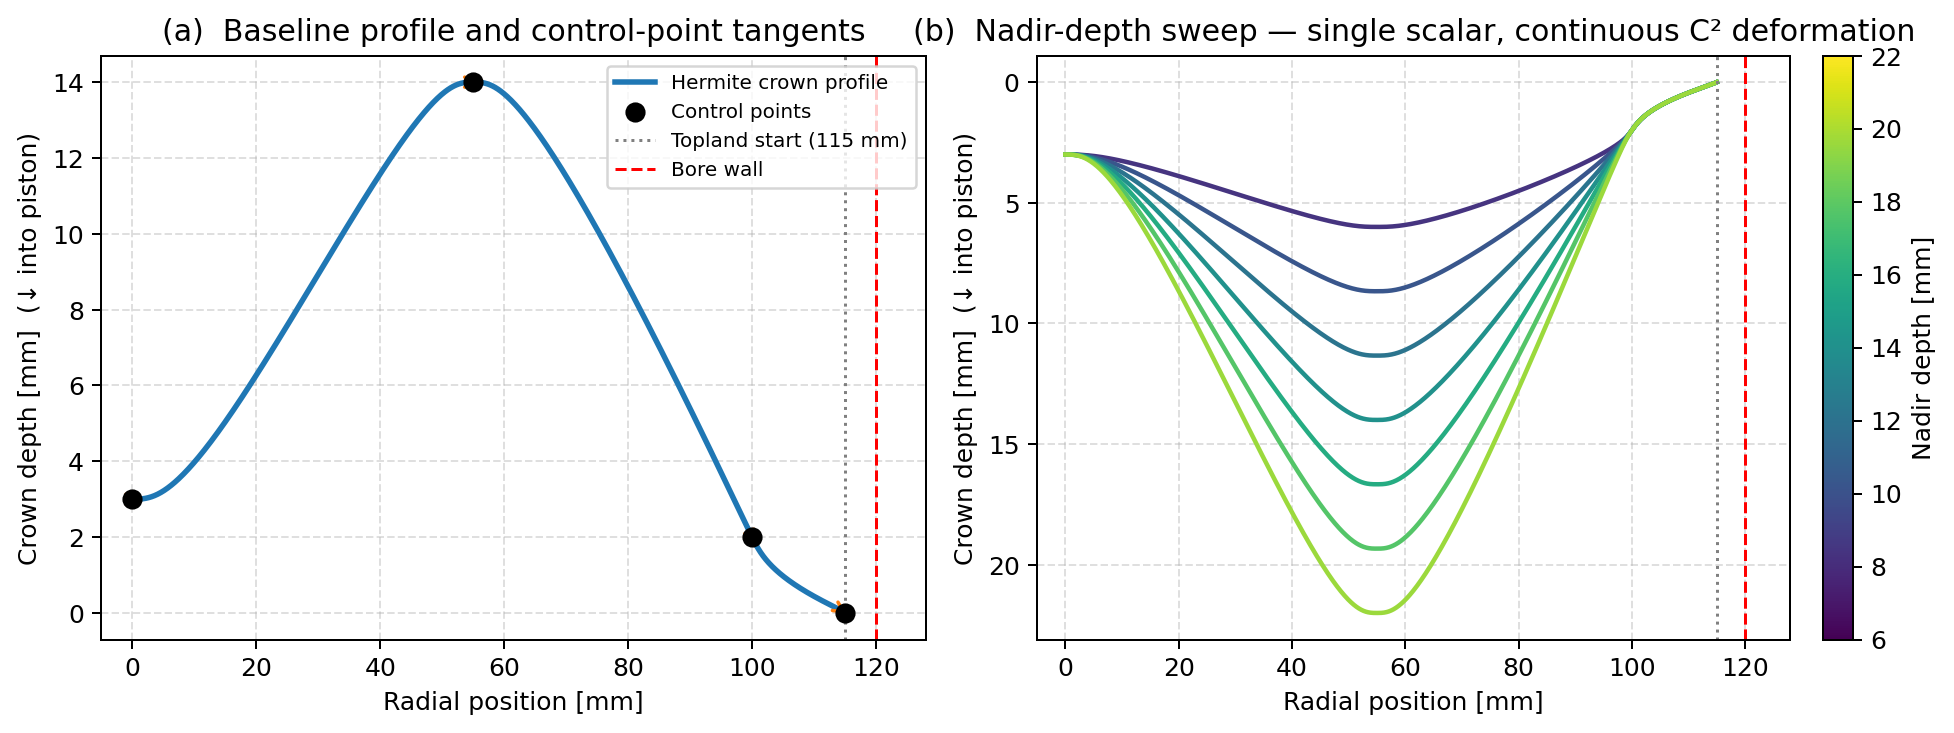
\includegraphics[width=0.96\linewidth]{images/hermite_crown_profile.png}
\caption{Quintic Hermite piston crown parameterisation. (a)~Baseline four-point profile; filled circles mark control points and orange arrows show the assigned tangent vectors. (b)~Nadir-depth sweep from \SI{6}{mm} to \SI{22}{mm}: varying one scalar continuously deforms the entire bowl profile while maintaining $C^{2}$ continuity across segment boundaries.}
\label{fig:hermite-crown}
\end{figure}

\textbf{Piston kinematics.}  The crown axial position follows the simplified slider-crank form \cite{HeywoodICE}
\[
h_{\mathrm{crown}}(t)=h_{0}-\tfrac{s}{2}\cos(\omega t+\varphi),\qquad \omega=\tfrac{2\pi\,\mathrm{RPM}}{60},
\]
where the implementation passes \(t\) in seconds to the angular-speed term while the GUI displays the time axis in milliseconds. This expression is the $r/l\to 0$ slider-crank limit and omits the higher-order connecting-rod correction. Phase $\varphi$ places the reference event at $t=0$. The default prototype setting of $\mathrm{RPM}=250$, $s/2=\SI{55}{mm}$, $h_{0}=\SI{75}{mm}$, and $\varphi=0$ corresponds to a short injection window close to top dead centre, over which the crown moves by less than \SI{1}{mm}; in this regime the connecting-rod correction is negligible.

\textbf{Per-frame collision integral.}  The instantaneous collision probability and the cumulative exposure over the injection window are
\[
P_{\mathrm{hit}}(t)=\iint p(x,y,t)\,\mathbf{1}_{\Omega_{\mathrm{piston}}(t)}(x,y)\,\mathrm{d}A,\qquad E=\int_{0}^{T} P_{\mathrm{hit}}(t)\,\mathrm{d}t,
\]
where \(\mathbf{1}_{\Omega_{\mathrm{piston}}(t)}\) is the binary indicator function for the instantaneous piston mask; the wall probability \(P_{\mathrm{wall}}(t)\) is computed by integrating the same PDF over the wall mask \(x\geq\SI{120}{mm}\). Spatial integration is performed on the canvas mesh, and cumulative exposure is computed by trapezoidal quadrature over the time grid. The side-channel onset-probability head from the distillation student is retained on the same time grid and plotted alongside $P_{\mathrm{hit}}(t)$ and \(P_{\mathrm{wall}}(t)\), so that the near-SOI onset confidence and the geometric interception probabilities can be read separately.

\textbf{Default output convention.}  The latest GUI artifact uses \(d_n=\SI{0.34}{mm}\), injection pressure \SI{2000}{bar}, chamber pressure \SI{15}{bar}, control back-pressure \SI{4}{bar}, 10 plumes, injection duration \SI{800}{\micro s}, fixed cone angle \(20^{\circ}\), and tilt angle \(20^{\circ}\). Over the 0--\SI{5}{ms} window, the non-negative mean used for plotting is \(\mu_{+}(t)\in[\SI{1.70}{mm},\,\SI{112.95}{mm}]\), the axial standard deviation is \(\sigma_{\parallel}(t)\in[\SI{4.39}{mm},\,\SI{17.66}{mm}]\), and the lateral standard deviation is \(\sigma_{\perp}(t)\in[\SI{0.50}{mm},\,\SI{6.64}{mm}]\). For the default Design~A run, the piston-hit probability peaks at \(P_{\mathrm{hit}}=0.7766\) at \(t=\SI{4.237}{ms}\), with \(P_{\mathrm{wall}}=0.0660\) in the same frame; the cumulative exposure over the full window is \(E=\SI{2.475}{ms}\), and the maximum wall probability is \(0.0857\). These values demonstrate that the end-to-end chain can propagate penetration distributions into ranked, time-resolved screening scores; they should not be interpreted as validated in-cylinder droplet impingement probabilities.

\textbf{Scope of the claim.}  The rotated-Gaussian envelope, the analytic cone-angle spread, and the slider-crank crown model are engineering simplifications, not resolved droplet-scale physics. This prototype is the probabilistic screening proxy argued for in the literature review; it is not a validated collision predictor against experimental high-speed footage or CFD collision fields.

The modelling workflow presented in this chapter --- from cleaned reduced-order targets through staged heteroscedastic training to probabilistic collision scoring --- constitutes the surrogate contribution of this thesis. A quantitative comparison of Stage~1, Stage~2, Stage~3, the physical baselines, and the sparse-GP alternative backbone on held-out test data, including coverage statistics and a leave-one-nozzle-family stress test, is presented in Chapter~5. The design decisions and their motivations are established here; the numerical payoff is reported there.
